\chapter{\emph{Modelling of Atg9}}
\section{Background}
The use of covariance methods to successfully predict key structural features that are possessed by the autophagy transmembrane protein Tmem41b and its DedA homologues led to the identification of another transmembrane autophagy protein to potentially structurally characterise; Atg9.  Like Tmem41b and Vmp1, Atg9 has been shown to function in the initiation stage of autophagasome formation at the endoplasmic reticulum \cite{Zhuang2017} and its structure and molecular physiological role was a mystery.

In autophagy, Atgs are proteins involved in autophagosome construction.  Atg9 is the only transmembrane Atg protein and is the first protein of the core autophagy machinery to arrive at the site of autophagosome construction.  Atg2 receives lipids from the endoplasmic reticulum (ER) and relays them to Atg9 which moves lipids between outer and inner layers of liposomes  resulting in growth of the phagophore which develops into an autophagosome \cite{sawa2020reconstitution,yamamoto2012atg9}.  Atg9 deficiency results in phenotypical features including abnormal ER expansion \cite{zhuang2017atg9}, cellular growth defects and impaired phagocytosis \cite{tung2010loss}. One copy of Atg9 is possessed by most organisms, however, there are examples of species where Atg9 has not been identified at all for example in Alveolata species \cite{aslan2017comparative,rigden2009autophagy}. There are two human Atg9 homologues; Atg9a and Atg9b.  Atg9b is restricted to fetal tissues as well as being present in placental tissues and tissues of the testes \cite{kusama2009comprehensive}. Atg9b has also be identified in certain cancer cell lines \cite{ma2017role,yun2020wnt}.  Atg9a is the predominant form and was the subject of the attempted structural characterisation described in this chapter.  Atg9 also functions as a regulator of the innate immune system where it attenuates the actions of STING thereby depressing the immune PRR/TBK1/IRF3 axis pathway \cite{imanishi2019reciprocal}.

Previous studies have shown that Atg9 is a multi-spanning transmembrane protein and have indicated that both the N- and C-termini are cytosolic with predictions that Atg9 possesses six transmembrane helices \cite{Young2006}. 


\section{Specific Methods}
\subsection{Transmembrane prediction}
TMHMM \cite{krogh2001predicting} was used to predict transmembrane helix regions of Atg9.  Although other methods such as TopCons are known to be more accurate \cite{Tsirigos2015}, TMHMM reports the probability that a region is in fact transmembrane rather than outputting a binary 'yes/no' designation.  The probability reporting feature of TMHMM was important here as there was the possibility of the presence of an unsuspected transmembrane helix within the accepted topology of Atg9. TMHMM uses algorithms for parameter estimation and transmembrane helix region prediction by utilising hidden Markov models (HMMs) describing hydrophobicity, charge bias, helix lengths, and grammatical constraints. 

\subsection{Homology modelling}
The potential homology between Atg9 and the transmembrane domain of Type I ABC transporters was used to construct homology models which provided potentially useful 3-D structures. The software Modeller \cite{eswar2006comparative} was used to predict the structure for Atg9 based on its sequence alignment with the transmembrane domain of two HHpred hits of Type I ABC transporters. Modeller used the sequence alignments as an input in addition to the atomic coordinates of the transmembrane domain of Type I ABC transporters, and a script file.  The script file loaded the 'AutoModel' class, created an 'AutoModel' object, and set the parameters to guide the model building procedure. The script also named the 'alnfile' that contained the Atg9-ABC alignment (in the PIR format) as well as defining the known ABC structure in the alignment file.  The last line of the script file called the make method and constructed the models. The output of Modeller was a calculated model containing all non-hydrogen atoms.  The validity of the models were evaluated by calculating the ResPre \cite{yang2019genetic} predicted contact satisfaction for the top L contacts. 

\subsection{Screening PDB for ABC Transporters}
A python script was written that search for and identified the key words 'ABC' or 'CASSETTE' in the title line of each of the PDB files of the PDB.  This resulted in 51 ABC structures being detected and being the approximate number of ABC transporters present in the PDB reported in the literature 
\cite{wilkens2015structure,hegedHus2021alphafold2}.

\section{Sequence Analysis}
Initial HHpred screening of the Atg9 sequence against the PDB \cite{Burley2018} using HHpred \cite{Zimmermann2018} reveals strong hits for the transmembrane domain (TMD) region with a number of several ABC transporters with the alignments covering the putative transmembrane domain of Atg9. The HHpred probabilities ranged from 50-20\%.  Additionally, all the ABC hits clustered at the top of the probability ranked results.

ABC transporters are a large superfamily \cite{rees2009abc} of integral membrane proteins that can be subdivided into a number of classes that show a high level of conservation in their nucleotide binding domains (NBDs).  The conservation of the NBD is in contrast to the transmembrane domain regions where great diversity is present in terms of both sequence and structure \cite{rees2009abc}. 

In order to assess the similarity of the transmembrane domains from the cluster of HHpred Atg9 ABC transporter hits, a Dali \cite{Holm2016} all-against-all comparison for these structures was performed.  The resulting Z-scores ranged from 19.5-31.3, showing clear structural similarity between these hits (figure \ref{fig:abc_comp}) supporting the idea that the Atg9 ABC transporter hits are probably not chance occurrences. 

%width=\textwidth
\begin{figure}[th!]
    \centering
    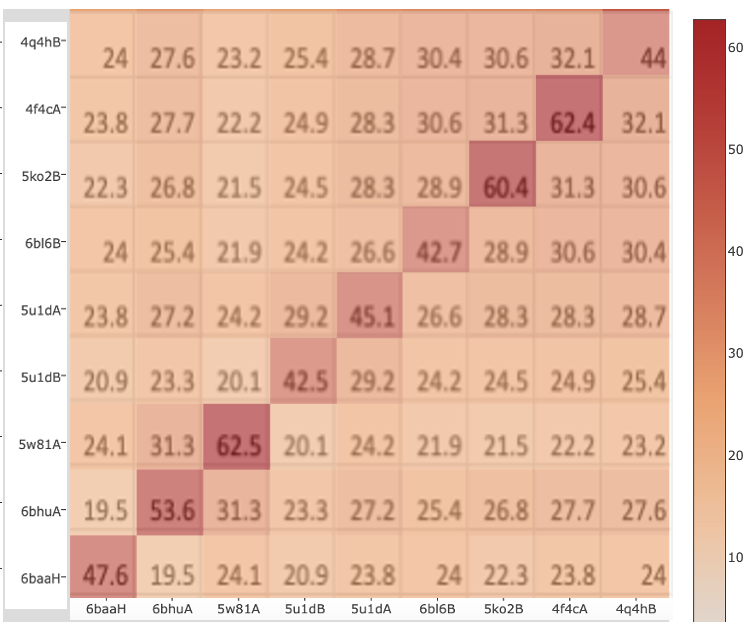
\includegraphics[width=90mm, scale=0.9]{Modelling of Atg9/abc_fold_comparison.png}
    \caption{Structural Alignments of ABC Transporter Hits}
    \label{fig:abc_comp}
    \small
    %Rosetta Ab initio Membrane model (magenta) structurally aligned with 5lilA (green).
\end{figure}


Querying the ABC transporters identified by HHpred against the Evolutionary Classification of Domain Boundaries (ECOD) database \cite{Cheng2014} indicated that all the ABC transporter hits were of Type 1 (Table \ref{ecod1}). 

\begin{table}
\caption{ECOD ABC Comparison}
\resizebox{\columnwidth}{!}{%
\centering
\arrayrulecolor{black}
\begin{tabular}{!{\color{white}\vrule}l!{\color{black}\vrule}l!{\color{black}\vrule}l!{\color{black}\vrule}l!{\color{black}\vrule}l!{\color{black}\vrule}l!{\color{black}\vrule}} 
\hline
\rowcolor[rgb]{0.267,0.447,0.769} \multicolumn{1}{!{\color{white}\vrule}c!{\color{black}\vrule}}{\textcolor{white}{\textbf{Domain ID~}}} & \multicolumn{1}{c!{\color{black}\vrule}}{\textcolor{white}{\textbf{X Group Name~}}} & \multicolumn{1}{c!{\color{black}\vrule}}{\textcolor{white}{\textbf{H Group Name~}}} & \multicolumn{1}{c!{\color{black}\vrule}}{\textcolor{white}{\textbf{T Group Name~}}} & \multicolumn{1}{c!{\color{black}\vrule}}{\textcolor{white}{\textbf{F Group Name~}}} & \multicolumn{1}{c!{\color{black}\vrule}}{\textcolor{white}{\textbf{Protein Name~}}}  \\ 
\hline
\rowcolor[rgb]{0.812,0.835,0.918} e5w81A4                                                                                                & Type II ABC exporter TMD fold                                      & Type I ABC exporter TMD fold                                       & Type I ABC exporter TMD fold                                       & ABC\_membrane                                                                       & Cystic fibrosis TM conductance regulator                                  \\ 
\hline
\rowcolor[rgb]{0.914,0.922,0.961} e4q4hA1                                                                                                & Type II ABC exporter TMD fold                                      & Type I ABC exporter TMD fold                                       & Type I ABC exporter TMD fold                                       & ABC\_membrane                                                                       & ABC transporter                                                                      \\ 
\hline
\rowcolor[rgb]{0.812,0.835,0.918} e4f4cA3                                                                                                & Type II ABC exporter TMD fold                                      & Type I ABC exporter TMD fold                                       & Type I ABC exporter TMD fold                                       & ABC\_membrane                                                                       & Multidrug Resistance Protein PGP-1                                                   \\ 
\hline
\rowcolor[rgb]{0.914,0.922,0.961} e3b5xA3                                                                                                & Type II ABC exporter TMD fold                                      & Type I ABC exporter TMD fold                                       & Type I ABC exporter TMD fold                                       & ABC\_membrane                                                                       & LIPID A Export ATP-binding/Permease Protein MSBA                                     \\ 
\hline
\rowcolor[rgb]{0.812,0.835,0.918} e5ko2A4                                                                                                & Type II ABC exporter TMD fold                                      & Type I ABC exporter TMD fold                                       & Type I ABC exporter TMD fold                                       & ABC\_membrane                                                                       & Multidrug resistance protein 1A                                                      \\ 
\hline
\rowcolor[rgb]{0.914,0.922,0.961} e5u1dA3                                                                                                & Type II ABC exporter TMD fold                                      & Type I ABC exporter TMD fold                                       & Type I ABC exporter TMD fold                                       & ABC\_membrane                                                                       & Antigen peptide transporter 1                                                        \\ 
\hline
\rowcolor[rgb]{0.812,0.835,0.918} e6bl6A2                                                                                                & Type II ABC exporter TMD fold                                      & Type I ABC exporter TMD fold                                       & Type I ABC exporter TMD fold                                       & ABC\_membrane                                                                       & Lipid A export ATP-binding/permease protein~MsbA                                     \\
\hline
\end{tabular}
}
\arrayrulecolor{black}
\label{ecod1}
\end{table}


Type 1 ABC transporters have transmembrane domains that are MetI-like.  The transmembrane domains of some of this group of ABC transporters are separate proteins \cite{kadaba2008high} from the nucleotide binding domain: this is exemplified by the methionine MetNI ABC transporter. This is in contrast to other type 1 ABC transporters such as ModBC and MalFGK where the NBD and TMD are one complete protein; these are generally larger and their subunits contain six transmemrane helices.  The homologous link between the two types of type 1 ABCs is recognised as the six helices correspond to the MetNI transporter where each MetI subunit is organised around a core of five transmembrane helices.  Utilising TMHMM, the Atg9 sequence was used to predict the number of TM helices (figure \ref{fig:atg9_tmhmm}).   TMHMM predicted six transmembrane helices, in line with type 1 ABC TMDs.  It should be noted that in addition to the strong predictions for the six TM helices, there was a low probability transmembrane prediction signal around residue 250. 

\begin{figure}[th!]
    \centering
    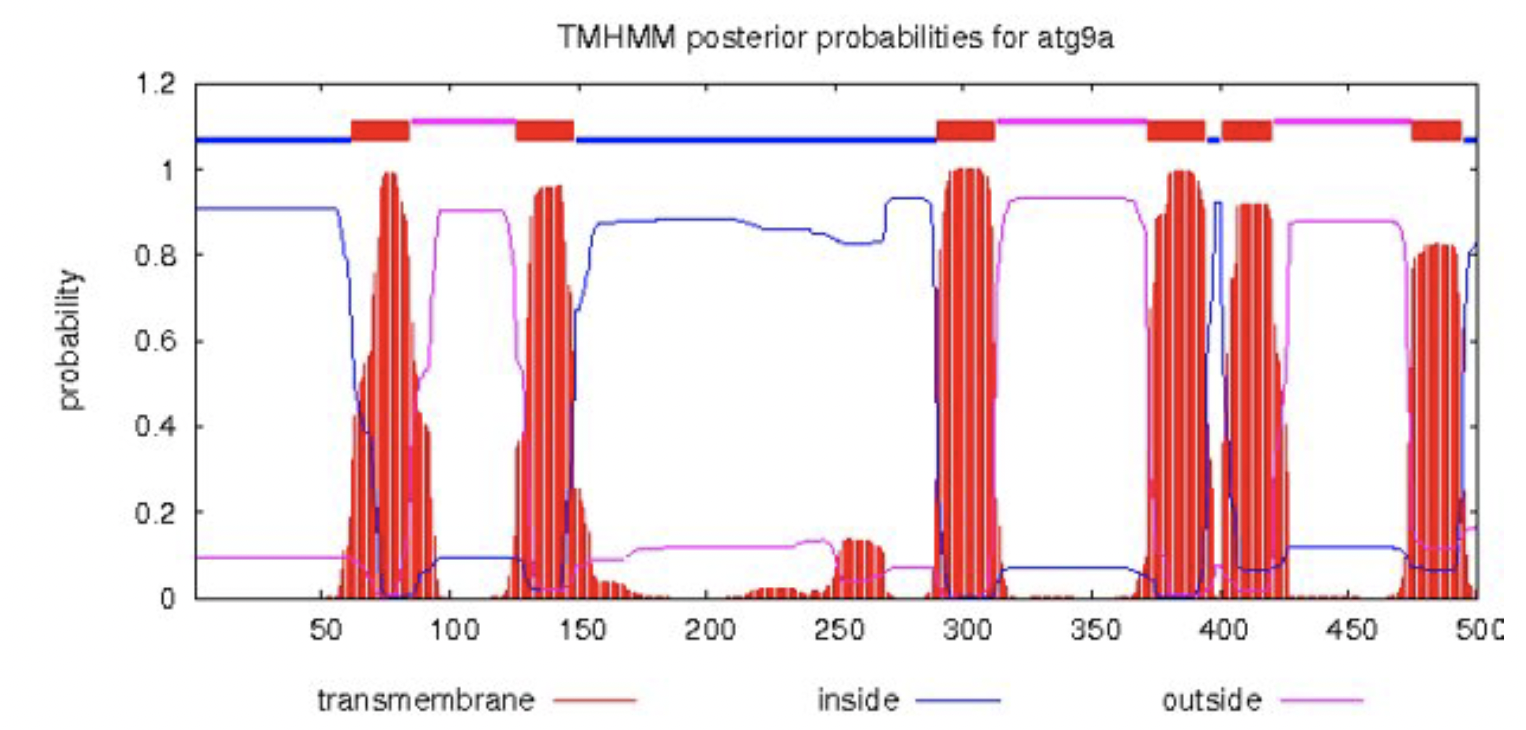
\includegraphics[width=90mm, scale=0.9]{Modelling of Atg9/atg9_tmhmm.png}
    \caption{TMHMM Prediction for TMD of Atg9}
    \label{fig:atg9_tmhmm}
    \small
    %Rosetta Ab initio Membrane model (magenta) structurally aligned with 5lilA (green).
    \label{fig:tmhmm}
\end{figure}


The combination of the HHpred probability scores and a lack of other good transmembrane protein matches in addition to the transmembrane topology prediction indicates that the Atg9 transmembrane region could very well have a Type 1 ABC transporter transmembrane domain - like fold.




To validate an ABC transporter-like fold for the putative transmembrane region of Atg9, the identification of any conserved key residues would be useful. Most ABC are transporters (importers or exporters) and all possess a nucleotide binding domain (NBD), at which hydrolysis of ATP provides the energy to drive the active transport. Atg9 does not contain the NBD sequence motifs and therefore obviously lacks NBD so unless it interacts non-covalently with an ATPase, Atg9 is not at least a conventional ABC transporter.  Conservation across the transmembrane domains of ABC transporters whose presence could be cross-referenced against Atg9 to validate the TMD ABC matches is not possible as the TMDs of the ABC superfamily are very diverse. Relating the observation of Atg9 having an ABC-like fold to its possible function is therefore not straightforward and cannot be accomplished by sequence analysis alone. Therefore, it was determined that three-dimensional modelling of Atg9 would be performed.  If modelled accurately, an ABC-like fold may be revealed, validating the ABC transporter link. 


\section{Homology Modelling}

Modeller was used to construct a homology model of the putative transmembrane domain of Atg9. The transmembrane domain of the top two HHpred hits were used as templates; 5w81 and 4q4h; with sequence similarities of 23\% and 24\% respectively. The sequence alignment was generated using ClustalW \cite{thompson2003multiple}. 

5w81 is the anion channel cystic fibrosis transmembrane conductance regulator CFTR. As with standard ABC transporters, CFTR is an active pump powered by ATP hydrolysis and possesses two transmembrane domains and two nucleotide-binding domains. CFTR is, however, atypical in that the channel gating in addition to ATP hydroysis also requires the phosphorylation of a cytosolic regulatory domain.  CFTR has two transmembrane and nucleotide-binding domains and is a single protein with each transmembrane domain containing six transmemtrane helices \cite{zhang2017conformational}. Figure \ref{fig:5w81_hmo} is the output 5w81 template homology model.


\begin{figure}[th!]
    \centering
    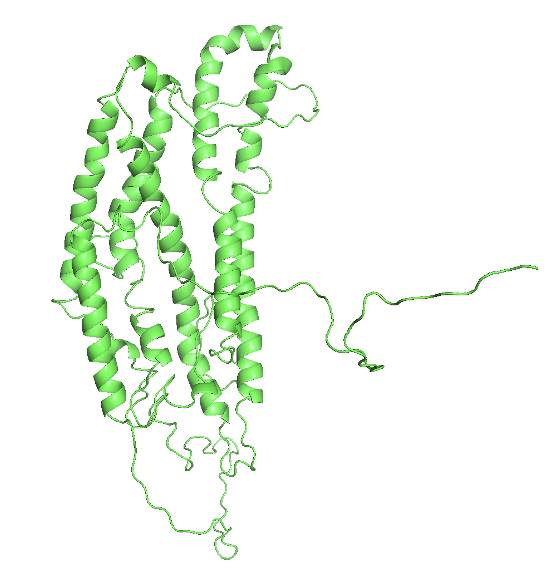
\includegraphics[width=50mm, scale=0.5]{Modelling of Atg9/atg9_hmo_5w81.png}
    \caption{Homology model for Atg9 (5w81 template)}
    \label{fig:5w81_hmo}
    \small
    %Rosetta Ab initio Membrane model (magenta) structurally aligned with 5lilA (green).
\end{figure}

\begin{figure}[htb]
    \centering % <-- added
\begin{subfigure}{0.5\textwidth}
  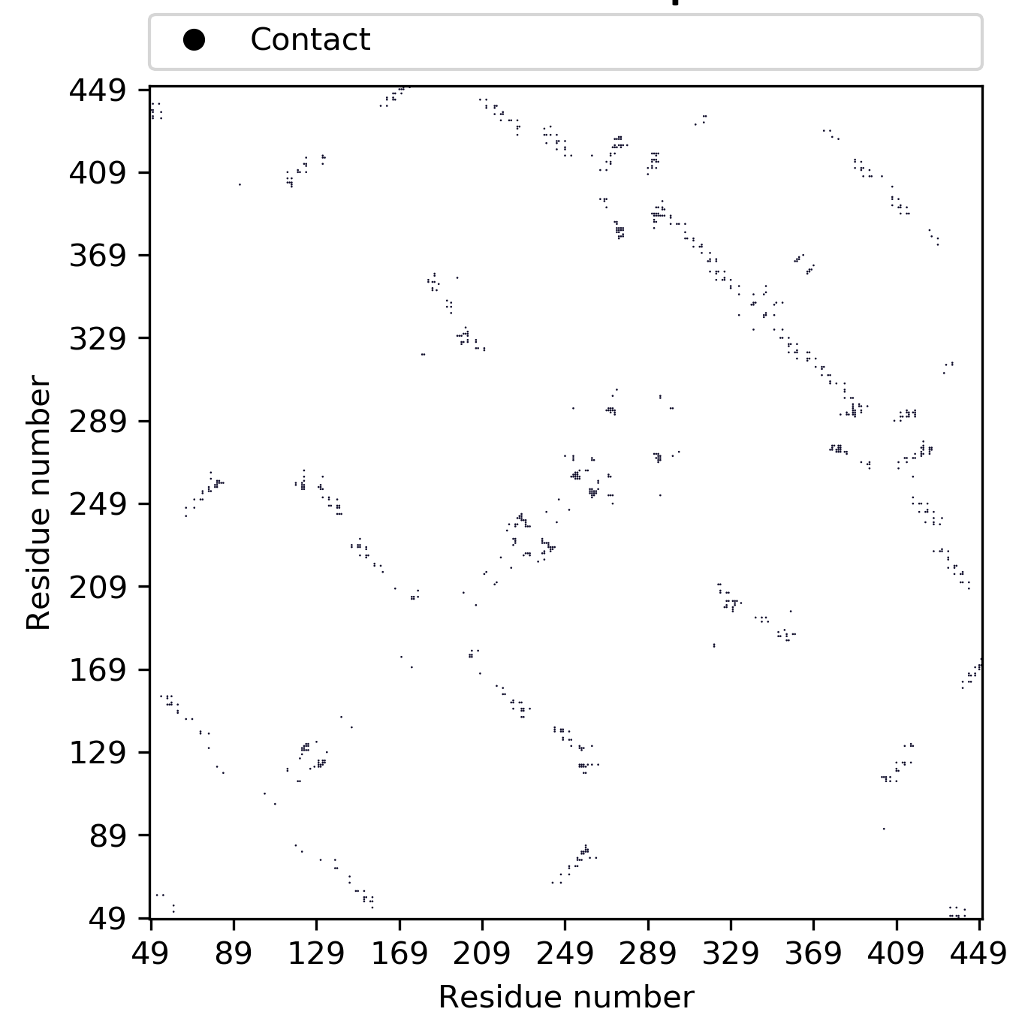
\includegraphics[width=\linewidth]{Modelling of Atg9/atg9_hmo_5w81_cmap.png}
  \caption{Atg9-5w81 Homology Model Contact Map}
  \label{fig:0}
  \end{subfigure}\hfil % <-- added
  \begin{subfigure}{0.45\textwidth}
  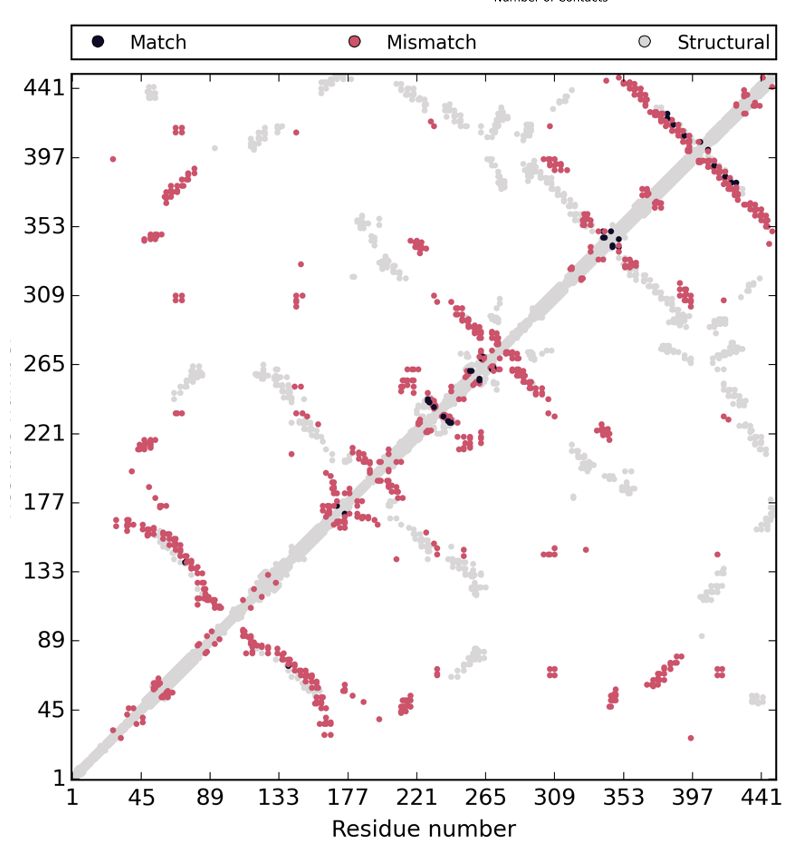
\includegraphics[width=\linewidth]{Modelling of Atg9/5w81_respre_super.png}
  \caption{Superposition of Atg9 ResPre predicted contacts with the Atg9-5w81 homology model}
  \label{fig:5w81_hom_cmap_super}
\end{subfigure}\hfil % <-- added
\begin{subfigure}{0.75\textwidth}
    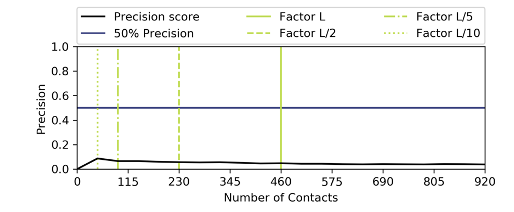
\includegraphics[width=\linewidth]{Modelling of Atg9/prec_5w81_respre.png}
    \caption{Precision profile of the Atg9 5w81 homology model}
    \label{fig:prec_5w81}
\end{subfigure}\hfil % <-- added
\caption{Atg9 5w81 Homology Model Quality Determination}
\small
\label{fig:atg9_5w81_quality}
\end{figure}


\begin{figure}[th!]
    \centering
    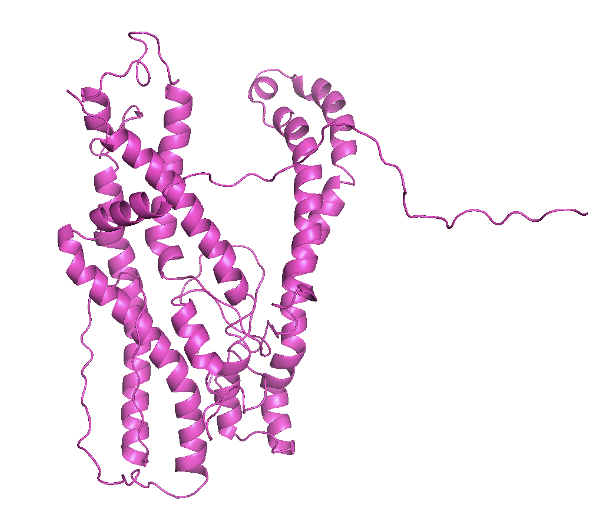
\includegraphics[width=50mm, scale=0.5]{Modelling of Atg9/atg9_hmo_4q4h.png}
    \caption{Homology model for Atg9 (4q4h template)}
    \label{fig:4q4h_hmo}
    \small
\end{figure}

A second homology model was constructed utilising 4q4h as a template. 4q4h is the crystal structure of TM287/288 ABC exporter and, like 5w81, possesses six transmembrane helices in each TMD \cite{hohl2014structural}.  Figure \ref{fig:4q4h_hmo} shows this output homology model.

\begin{figure}[htb]
    \centering % <-- added
\begin{subfigure}{0.5\textwidth}
  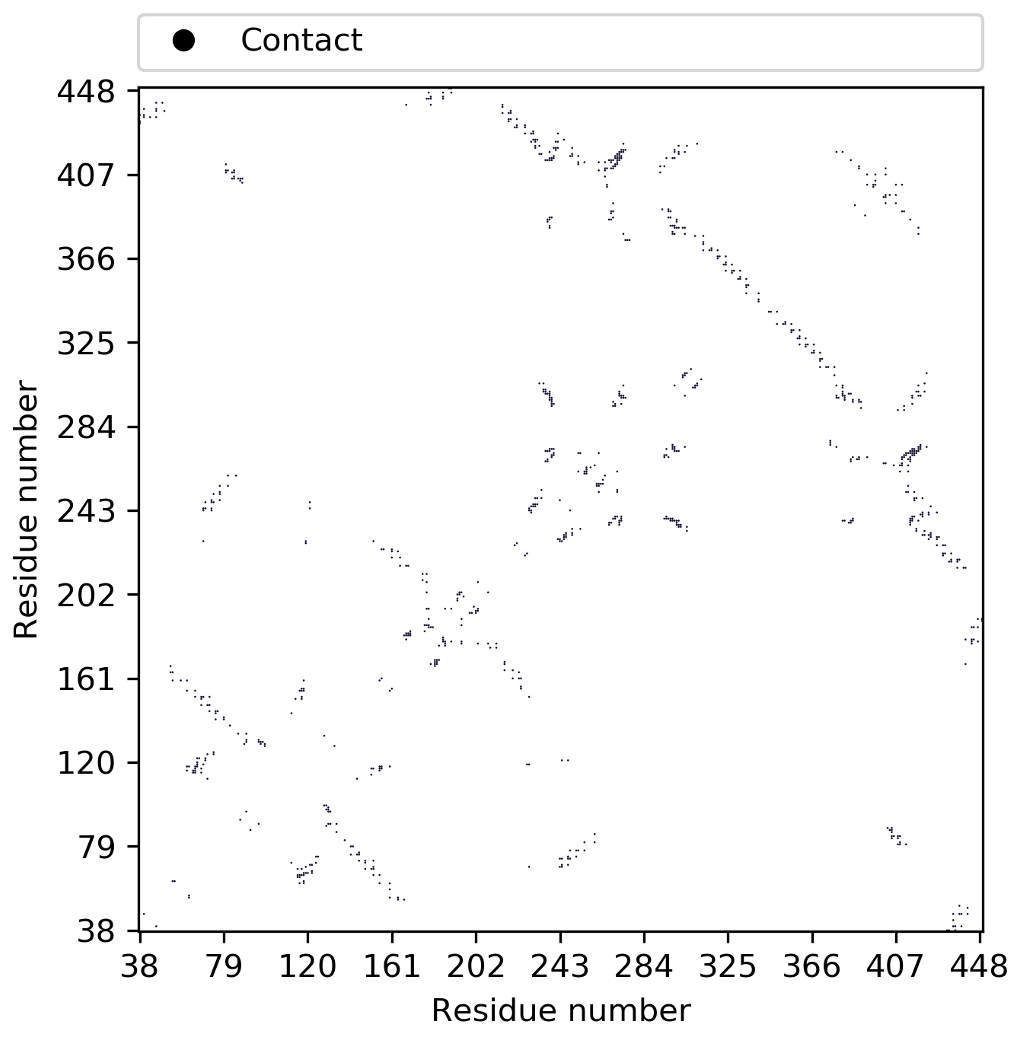
\includegraphics[width=\linewidth]{Modelling of Atg9/atg9_hmo_4q4h_cmap.png}
  \caption{Atg9 4q4h Contact Map}
  \label{fig:0}
\end{subfigure}\hfil % <-- added
\begin{subfigure}{0.45\textwidth}
  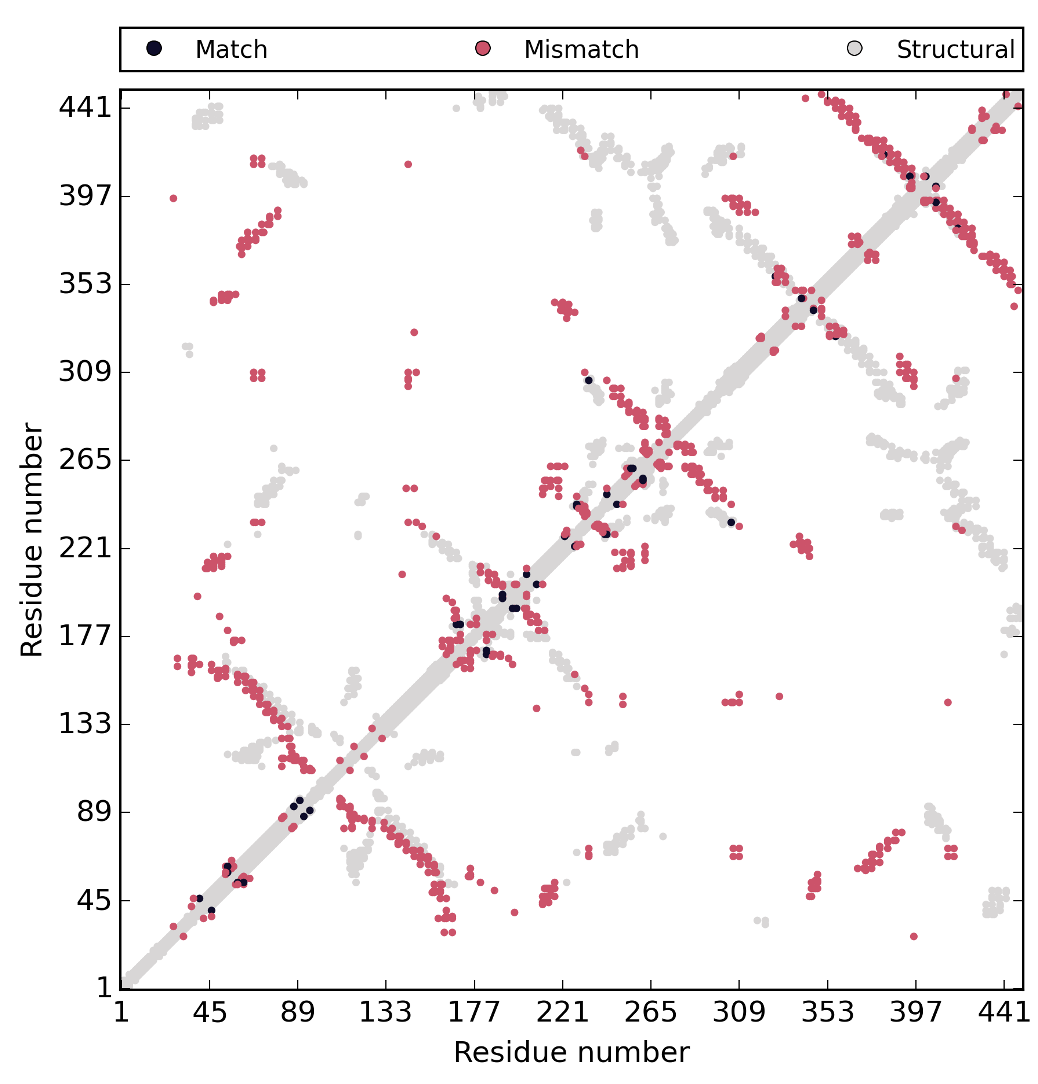
\includegraphics[width=\linewidth]{Modelling of Atg9/super_atg9_hmo_4q4h.png}
  \caption{Superposition of ResPre predicted contacts with 4q4h homology model}
  \label{fig:4q4h_hom_cmap_super}
\end{subfigure}\hfil % <-- added
\begin{subfigure}{0.75\textwidth}
  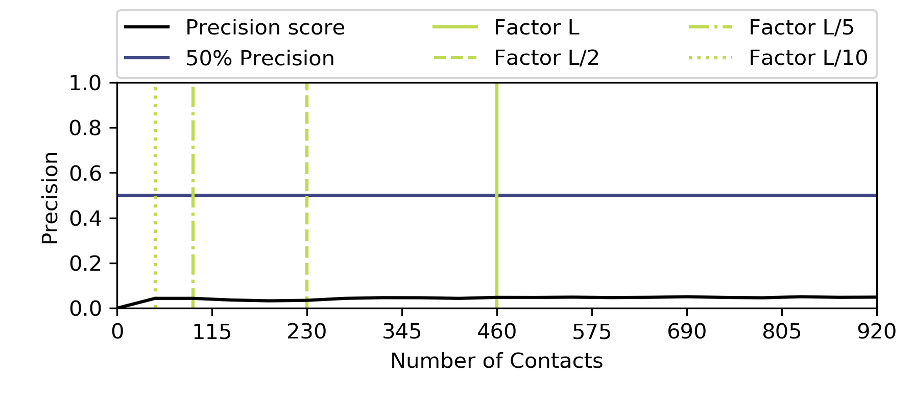
\includegraphics[width=\linewidth]{Modelling of Atg9/prec_hmo_4q4h.png}
  \caption{Precision profile of the Atg9 4q4h homology model}
  \label{fig:prec_4q4h}
\end{subfigure}\hfil % <-- added
\caption{Atg9 4q4h homology model quality determination}
\small
\label{fig:atg9_4q4h_quality}
\end{figure}

Performing the predicted contact satisfaction analysis \cite{Simkovic2017} for both homology models revealed a poor contact satisfaction profile indicating that the correct fold of Atg9 was not achieved through the homology modelling exercise (figures \ref{fig:prec_5w81} and \ref{fig:prec_4q4h}).  In an effort to determine whether there were any local regions where the modelling had captured the correct fold, the contact maps derived from the ResPre \cite{yang2019genetic} predictions and the homology models were superposed (figures \ref{fig:5w81_hom_cmap_super} and \ref{fig:4q4h_hom_cmap_super}).  The superpositions did hint at common features (Figures \ref{fig:5w81_hom_cmap_super} and \ref{fig:4q4h_hom_cmap_super}).  The figures use the homology model as the reference structure; grey points are homology model contacts not present in the predicted contact map while black points are contacts present in both model and prediction; red points are contacts present in the prediction but not in the model. Analysis proved difficult; it was problematic to ascertain whether the contact map features were by virtue of alpha helical contacts and therefore not indicative of homology or whether local structural features had actually been actually correctly folded.

\section{Ab initio Modelling}
The unsuccessful Atg9 homology modelling trial led to an attempt to construct ab initio models for Atg9 in an effort to test the hypothesis that Atg9 possesses an ABC-like fold. A metagenomics-enriched database was employed to obtain as accurate as possible covariance-based contact predictions.  The use of the metagenomics database to build the MSA for Atg9 was successful in raising the Neff from 438 (using Uniprot) to 843 for the whole protein. The sequence coverage profile showed that the number of sequences in the MSA covering the C-terminal side after position remain low (Figure \ref{fig:atg9_msa}).  The boundary at position 500 represents the end of the first domain; indeed, HHpred alignments of Atg9 show the Type I ABC transporters transmembrane domains matching with this first putative domain.  Calculating the Neff values for this first domain gave values of 554 when using Uniprot and 1024 when utilising the metagenomics database. JackHMMER \cite{Johnson2010} was then used to generate the MSAs and ResPre \cite{Li} to make the contact predictions based on the metagenomics enhanced MSAs for the putative transmembrane domain of Atg9.  The predicted contact information was then used as restraints to construct models using both Rosetta ab initio and RosettaMembrane protocols.  TopCons transmembrane predictions were also used as restraints for RosettaMembrane model building.  One thousand models of each were constructed and each of the thousand were clustered using Spicker; the centroid of the largest cluster was selected as the top model.  RosettaMembrane models contained a number of larger clusters with the maximum cluster size being 200 and the smallest cluster being 68.  This is in contrast to the clustering of the Rosetta ab initio models where cluster sizes were much smaller with the maximum cluster size being five and the smallest clusters being only two, indicating that the output models did not converge on a consensus energetic minimum.  

\begin{figure}[htb]
\begin{subfigure}{0.5\textwidth}
  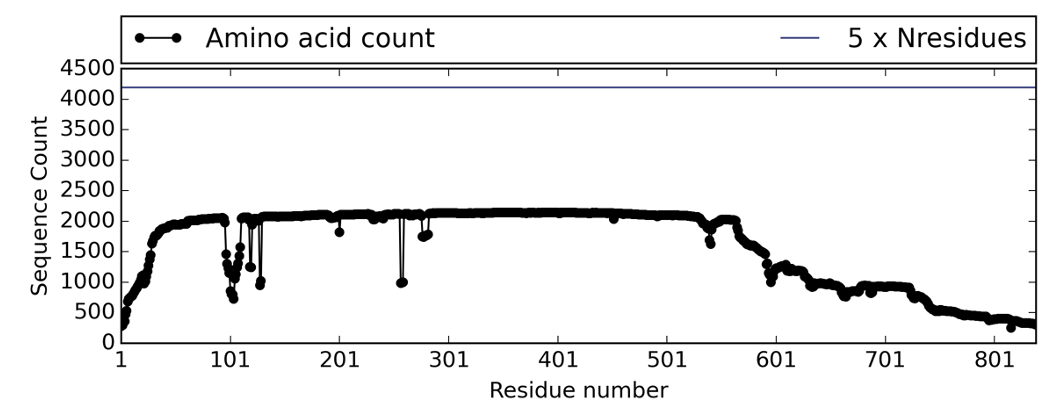
\includegraphics[width=\linewidth]{introduction/atg9_mas_uni.png}
  \caption{Atg9 Uniprot MSA coverage}
  \label{fig:0}
\end{subfigure}\hfil % <-- added
\begin{subfigure}{0.5\textwidth}
  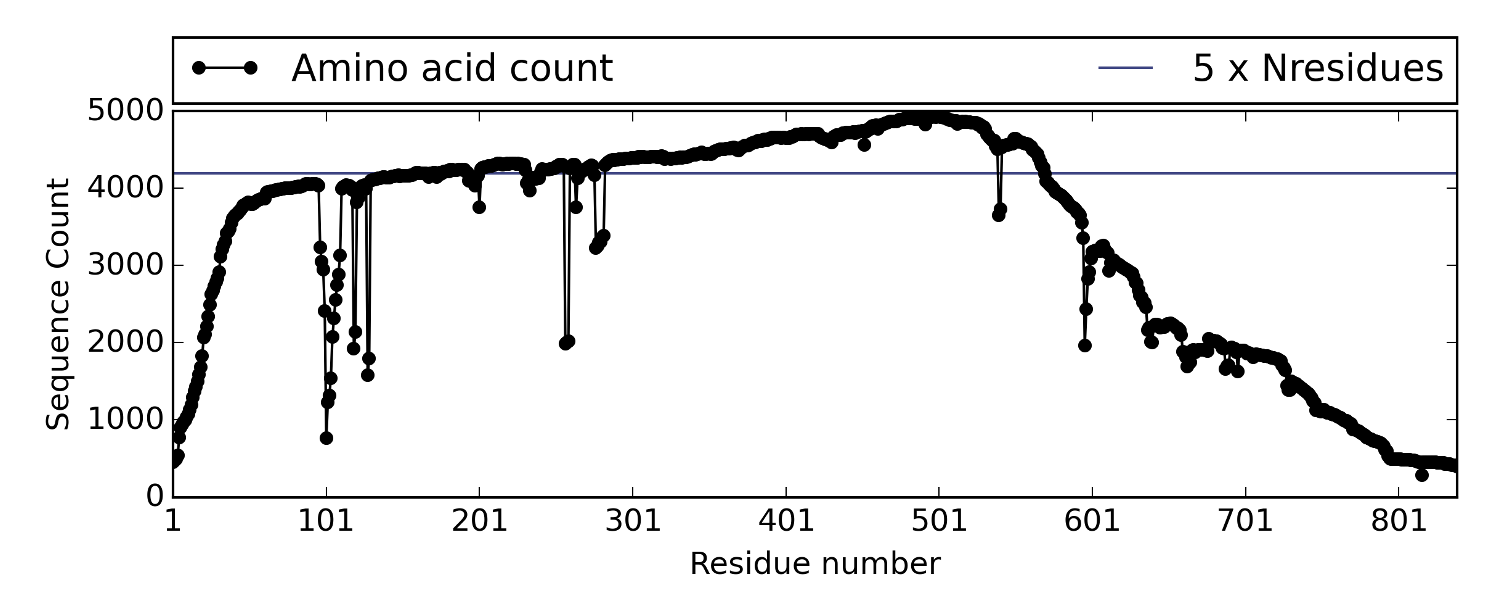
\includegraphics[width=\linewidth]{introduction/atg9_msa_meta.png}
  \caption{Atg9 metagenomic MSA coverage}
  \label{fig:1}
\end{subfigure}\hfil % <-- added
\caption{Atg9 MSA Sequence coverage profiles}
\small
\label{fig:atg9_msa}
\end{figure}

The output models from the RosettaMembrane flavour appeared more plausible compared to the outputs from Rosetta ab initio;  these models possessed helices packed together in such a way that they could conceivably sit in a membrane bi-layer.  Indeed running the top model against the PDB using DALI did result in three ABC transporter hits albeit of the Type II class; 6quz-D (z=3.9), 2lw1-A (z=5.4),  and 4MRN-B (z=6).  Despite the fact that the resultant RosettaMembrane models appeared visually promising and good PDB structural hits with ABC transporters, quantitative analysis of both the Rosetta ab initio and the RosettaMembrane  structural predictions resulted in poor precision scores (Figure \ref{fig:atg9_ab_models}) indicating that the correct fold had not been predicted \cite{DeOliveira2016}.

\begin{figure}[htb]
    \centering % <-- added
\begin{subfigure}{0.25\textwidth}
  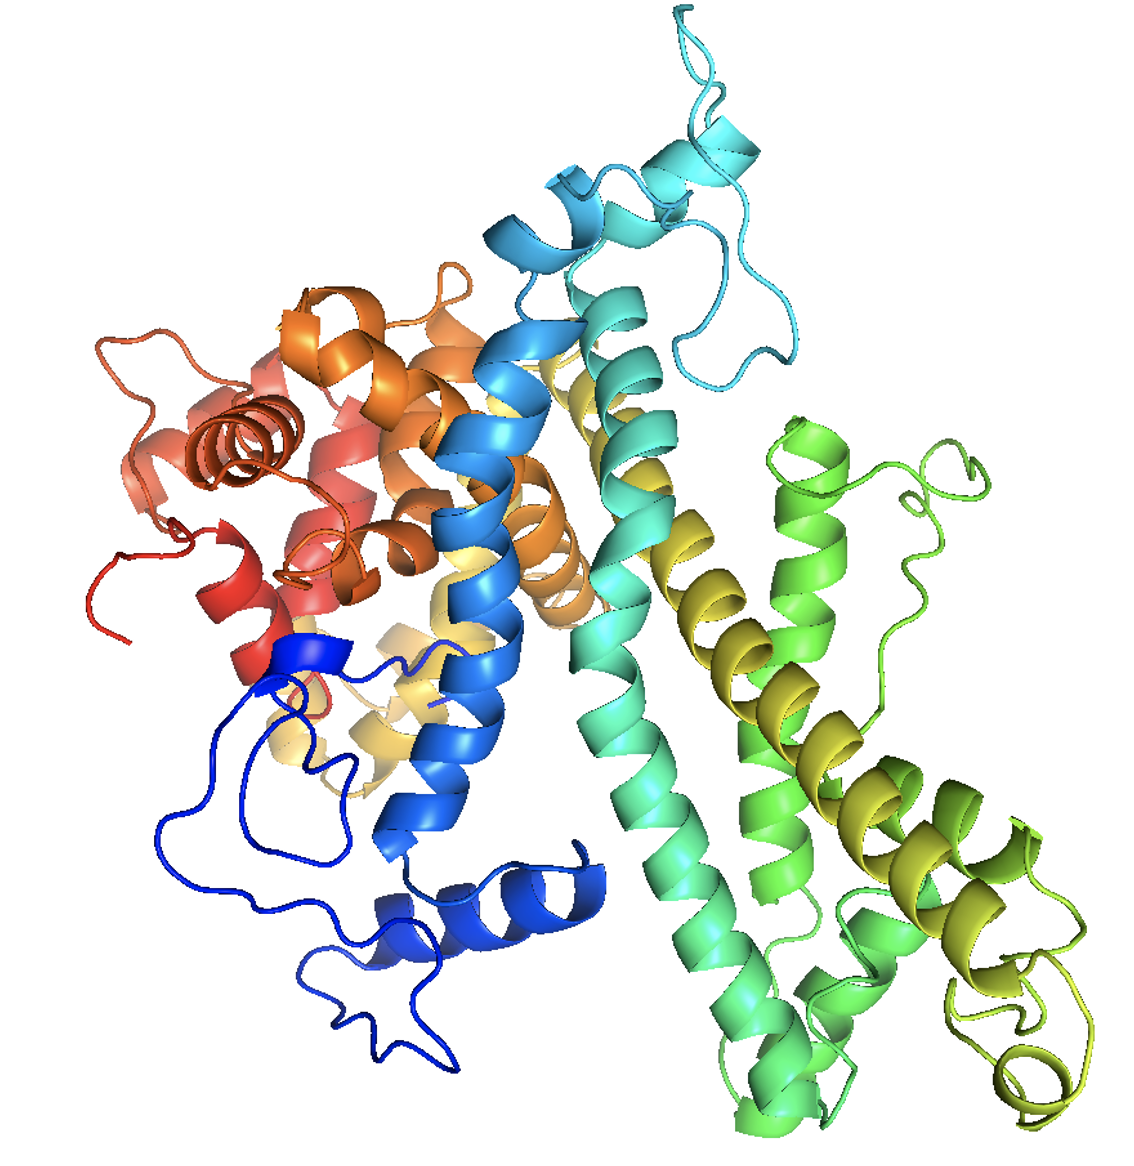
\includegraphics[width=\linewidth]{Modelling of Atg9/atg_ros_ab.png}
  \caption{Rosetta Ab initio model of Atg9 TMD}
  \label{fig:0}
\end{subfigure}\hfil % <-- added
\begin{subfigure}{0.25\textwidth}
  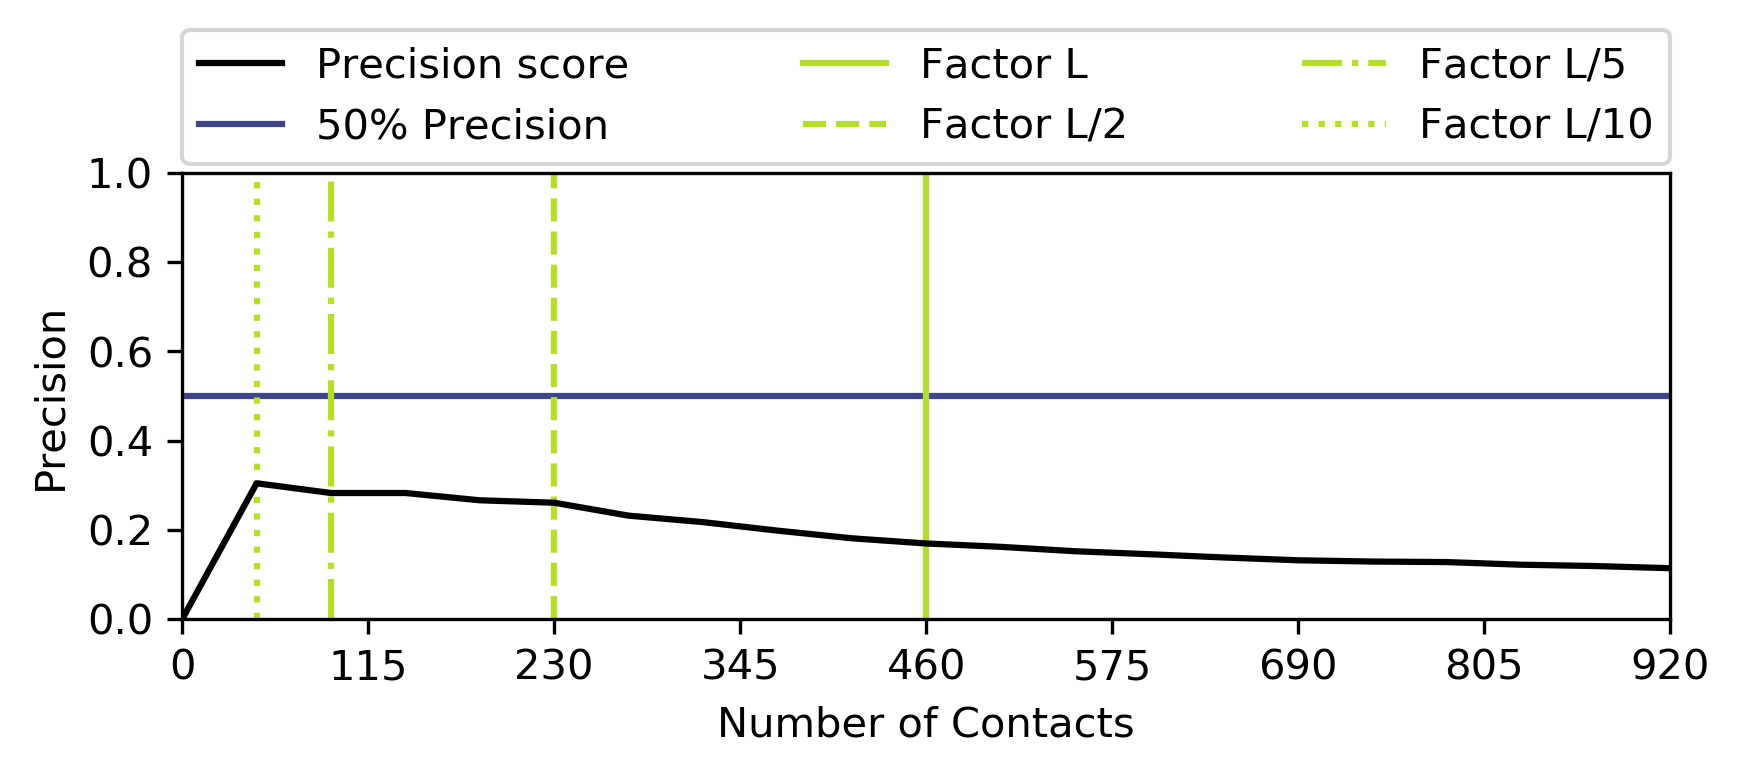
\includegraphics[width=\linewidth]{Modelling of Atg9/prec_ros.png}
  \caption{Precision profile of Rosetta Ab initio model of Atg9 TMD}
  \label{fig:0}
\end{subfigure}\hfil % <-- added
\begin{subfigure}{0.25\textwidth}
  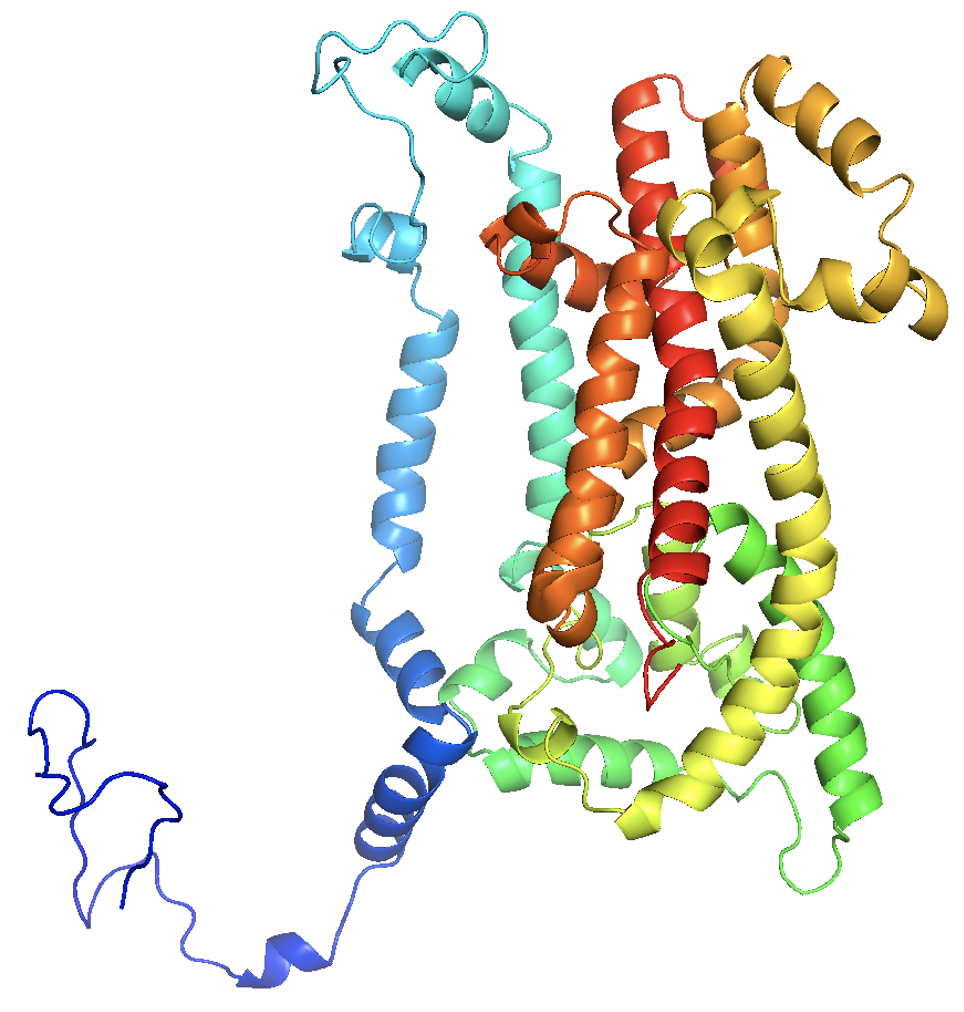
\includegraphics[width=\linewidth]{Modelling of Atg9/atg_ros_mem.png}
  \caption{RosettaMembrane model of Atg9 TMD}
  \label{fig:1}
\end{subfigure}\hfil % <-- added
\begin{subfigure}{0.25\textwidth}
  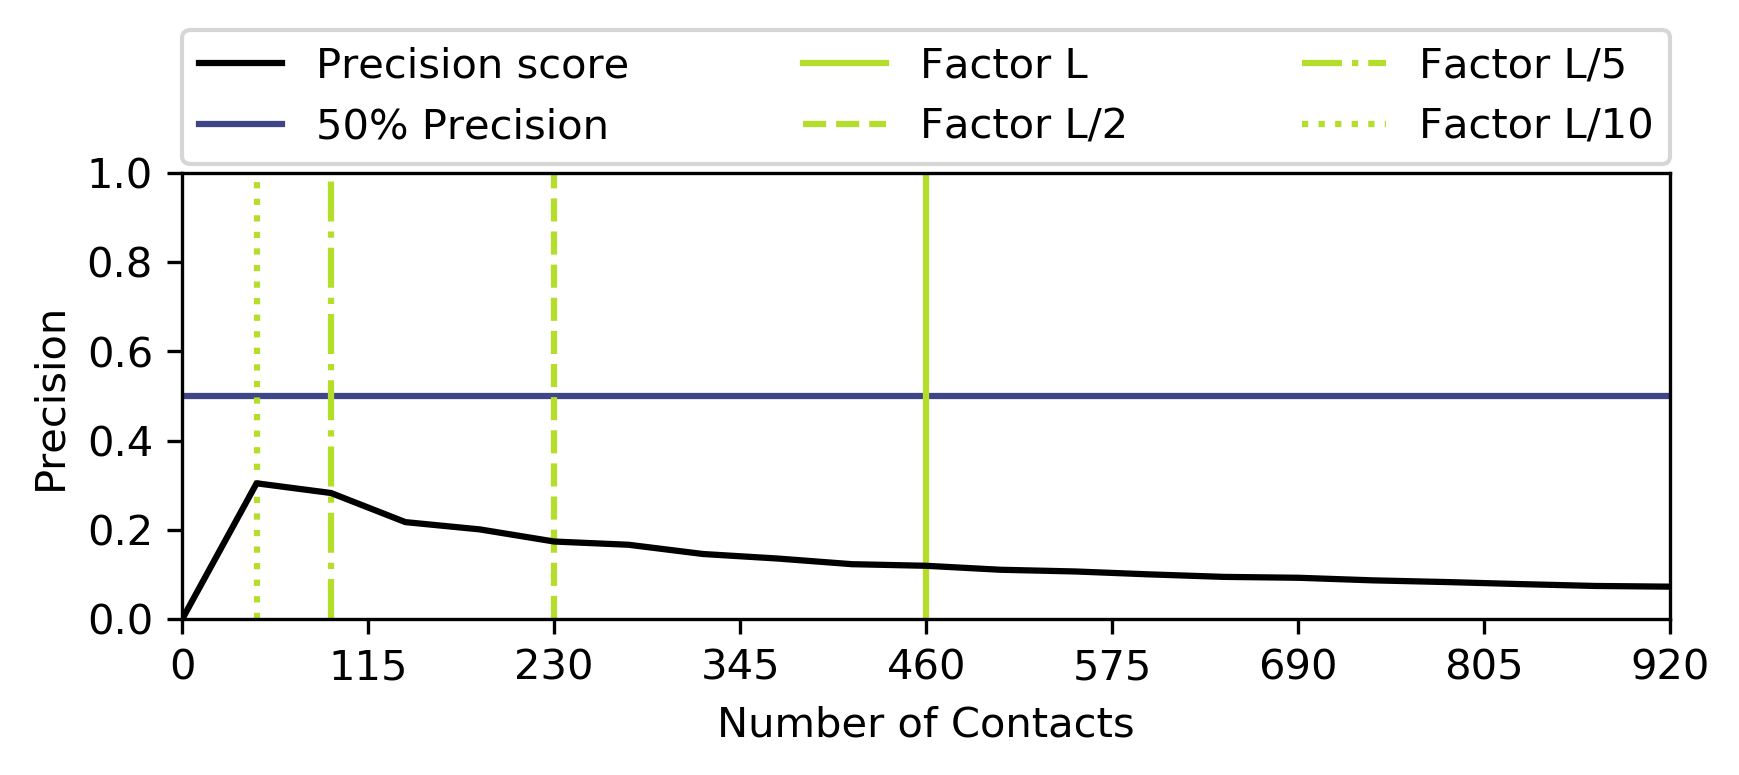
\includegraphics[width=\linewidth]{Modelling of Atg9/prec_rosmem.png}
  \caption{Precision profile of Rosetta Ab initio model of Atg9 TMD}
  \label{fig:0}
\end{subfigure}\hfil % <-- added
\caption{Ab initio modelling of Atg9}
\small
Precision score evaluation of the Rosetta ab initio and RosettaMembrane model in relation to the predicted contacts at various contact cutoff values are shown where L = sequence length (rounded down to the nearest whole number of contacts). The 50\% precision cut off is shown (blue line) as a visual marker. A minimum of 70\% contact satisfaction for the top L contacts would be suggestive of good quality models \cite{DeOliveira2016}.
\label{fig:atg9_ab_models}
\end{figure}

\section{Contact Map Analysis}
Efforts to obtain evidence of Atg9 and Type I ABC tranporter transmembrane domain homology independent of the HHpred results using homology and ab initio modelling did not yield convincing data.  In the case of ab initio modeling this was to be expected as trying to make accurate structural prediction for a 500 residue protein was, at the time, uncommon as large complex proteins present a convergence challenge for ab initio structure prediction (Figure \ref{fig:croem_vs_5w81}). The idea of successful ab initio modelling was relying heavily on the contact predictions acting as restraints.  Knowing that the contact predictions are very reliable an alternative tool was identified that could screen the PDBTM utilising the contact information by passing the need to structurally predict the structure of Atg9; MapAlign \cite{Ovchinnikov2017}. 

MapAlign was developed in 2017 by the Baker group as a tool to refine the structures of ab initio models.  MapAlign was used to identify contact map feature matches to known structures and aid the modelling of large and complex proteins that otherwise would be a challenge for ab initio structure prediction. MapAlign exploits the fact that structural matches can be detected by covariance analysis in the absence of detectable sequence similarity since structural similarity is retained over larger evolutionary distances.  MapAlign was used to screen predicted contacts against of the PDB; performing contact-based structure matching by comparing contact maps of the query and target and attempting to align predicted contacts with the contact patterns of experimental structures then highlighting any structural matches. In its original implementation, the matches were then used to refine the ab initio models.  MapAlign compares two contact maps and returns an alignment that attempts to maximize the number of overlapping contacts at the same time as attempting to minimise the number of gaps.

MapAlign was employed to screen the predicted contacts of the putative transmembrane domain of Atg9 against a library of non-redundant PDBTM structures. The input contact predictions for Atg9 were filtered to leave only the medium (above six residues apart) and long range (above twelve residues apart) contacts; this step was taken as the successful usage of MapAlign by the GREMLIN group only utilised these sets of predicted contacts when employing this contact map alignment tool \cite{Ovchinnikov2017} and therefore may have been optimised for these contact categories. 

MapAlign provided a list of the 25 top hits ranked by the MapAlign score (a combination of contact satisfaction and gap penalties).  The top 25 results listed PDBTM hits that seemed not to be related in any way and there was no clustering of related proteins at the top of the list.  Within the top 25 hits there were, however, six ABC transporter hits (Figure  \ref{table:map_align_eco}) that, according to the Evolutionary Classification of Protein Domains (ECOD), were all of the Type II class.

\begin{table}
\caption{ECOD classification comparison of the ABC transporter MapAlign hits}
\resizebox{\columnwidth}{!}{%
\centering
\arrayrulecolor{black}
\begin{tabular}{!{\color{white}\vrule}l!{\color{black}\vrule}l!{\color{white}\vrule}l!{\color{white}\vrule}l!{\color{white}\vrule}l!{\color{white}\vrule}l!{\color{white}\vrule}} 
\hline
\rowcolor[rgb]{0.267,0.447,0.769} \multicolumn{1}{!{\color{white}\vrule}c!{\color{black}\vrule}}{Domain ID~} & \multicolumn{1}{c!{\color{white}\vrule}}{X Group Name~} & \multicolumn{1}{c!{\color{white}\vrule}}{H Group Name~} & \multicolumn{1}{c!{\color{white}\vrule}}{T Group Name~} & \multicolumn{1}{c!{\color{white}\vrule}}{F Group Name~} & \multicolumn{1}{c!{\color{white}\vrule}}{Protein Name~}                \\ 
\hline
\rowcolor[rgb]{0.812,0.835,0.918} e5l22A2                                                                    & Type II ABC exporter TMD fold          & Type I ABC exporter TMD fold           & Type I ABC exporter TMD fold           & ABC\_membrane                                           & ABC transporter (HlyB subfamily)                                       \\ 
\hline
\rowcolor[rgb]{0.914,0.922,0.961} e5mkkA2                                                                    & Type II ABC exporter TMD fold          & Type I ABC exporter TMD fold           & Type I ABC exporter TMD fold           & ABC\_membrane                                           & Multidrug resistance ABC transporter ATP-binding and permease protein  \\ 
\hline
\rowcolor[rgb]{0.812,0.835,0.918} e5eg1A2                                                                    & Type II ABC exporter TMD fold          & Type I ABC exporter TMD fold           & Type I ABC exporter TMD fold           & ABC\_membrane                                           & Microcin-J25 export ATP-binding/permease protein McjD                  \\ 
\hline
\rowcolor[rgb]{0.914,0.922,0.961} e4aywA2                                                                    & Type II ABC exporter TMD fold          & Type I ABC exporter TMD fold           & Type I ABC exporter TMD fold           & ABC\_membrane                                           & ATP-BINDING CASSETTE SUB-FAMILY B MEMBER 10                            \\ 
\hline
\rowcolor[rgb]{0.812,0.835,0.918} e4mrnA1                                                                    & Type II ABC exporter TMD fold          & Type I ABC exporter TMD fold           & Type I ABC exporter TMD fold           & ABC\_membrane                                           & ABC TRANSPORTER RELATED PROTEIN                                        \\ 
\hline
\rowcolor[rgb]{0.914,0.922,0.961} e3wmfA2                                                                    & Type II ABC exporter TMD fold          & Type I ABC exporter TMD fold           & Type I ABC exporter TMD fold           & ABC\_membrane                                           & ATP-binding cassette, sub-family B, member 1                           \\ 
\hline
\rowcolor[rgb]{0.812,0.835,0.918} e4ry2A3                                                                    & Type II ABC exporter TMD fold          & Type I ABC exporter TMD fold           & Type I ABC exporter TMD fold           & ABC\_membrane                                           & ABC-type bacteriocin transporter                                       \\
\hline
\end{tabular}
}
\label{table:map_align_eco}
\arrayrulecolor{black}
\end{table}

The use of the contact map alignment method MapAlign again did not provide definitive hits that would indicate a common co-evolutionary profile between Atg9 and Type I ABC transporter transmembrane domains. 

A major issue with both the ab initio modelling and attempted contact map alignment methods is that even with good co-variance information the biologically
important contacts it reveals will be a superposition of contacts from different conformational states and if it is an oligomer, intra- and inter-molecular contacts would also be present; if Atg9 is indeed an oligomeric transporter then both of these would result in noise when attempting to model or align contact maps.


\section{Analysis: Low Resolution CryoEM Model}

During the investigation into Atg9 a low resolution (7.8Å) CryoEM structure of Arabidopsis Atg9 was published \cite{Lai2020}.  The group combined contact prediction using co-evolutionary data to construct a model and claim insight into the Atg9 architecture.  The group concludes that Atg9 has six transmembrane $\alpha$-helices and forms a homotrimer where at the center, the protomers interact via their membrane-embedded and C-terminal cytoplasmic regions. 

The published material gave another possible avenue to determine the molecular function of Atg9 and whether it is related to Type I ABC transporters.  The conclusion that Atg9 forms a homo-trimer is in conflict with the possibility of the ABC transporter link as there are no ABC transporters that function by forming a trimer; although this could still be possible if Atg9 is only distantly related to ABCs and not explicitly a member of the ABC transporter super family. Careful examination of the data presented in the paper indicate that the authors' conclusions are speculative as the experimental interpretation is dependent on the bioinformatics at this resolution.  The team utilised RaptorX \cite{Ma2015} to generate the covariance-derived contact predictions, again, the paper does not show the predicted contact map to demonstrate the strength of the inter-helical predictions that are the key information that allowed them to tentatively trace the transmembrane helices. Analysing the data further presented in the paper the authors state that "the final model places C$\alpha$ of the pairwise residues are within 15 Å of each other in 43 out of the top 46 identified pairs, with an average distance of 10.2 Å. The 7\% violated C$\alpha$- C$\alpha$ distance constraints is in agreement with the observed false-positive rate in previous structure prediction studies of known protein structures using evolutionary covariance."; 15Å was a very generous threshold as contact prediction methods are usually bench-marked with C$\beta$ (not C$\alpha$) within 8Å.  This analysis leads to the possibility that the resolution of the EM-map coupled with information gained from the model of Atg9 was insufficient to dock predicted model in the map as they based their speculation from only small amounts of data. For example, in the section titled the cytoplasmic region:

'Consequently, we ascribe the remaining density in our reconstruction to largely represent the structured domains of the C-terminal regions. The estimated volume of this region is 20\% of the density of the entire protomer, which approximately corresponds to the size of a 20 kDa polypeptide and is consistent with the calculated mass of the structured domain (16 kDa). The C-terminal region forms three distinct petal-shaped features around the three-fold axis where the middle loop is tucked behind.'

The structure and the proceeding docking should have been verified; this could have been achieved by using domain (N- or C- terminal) specific antibodies to label these regions in the single particle reconstruction or alternatively use the tagging before going onto structure prediction and docking; this may have improved the particle alignments and resolution. Consequently the experimental data does not offer much constrain to the structure prediction and docking therefore it is only as good as the bioinformatic predictions that were applied.

\begin{figure}[th!]
    \centering
    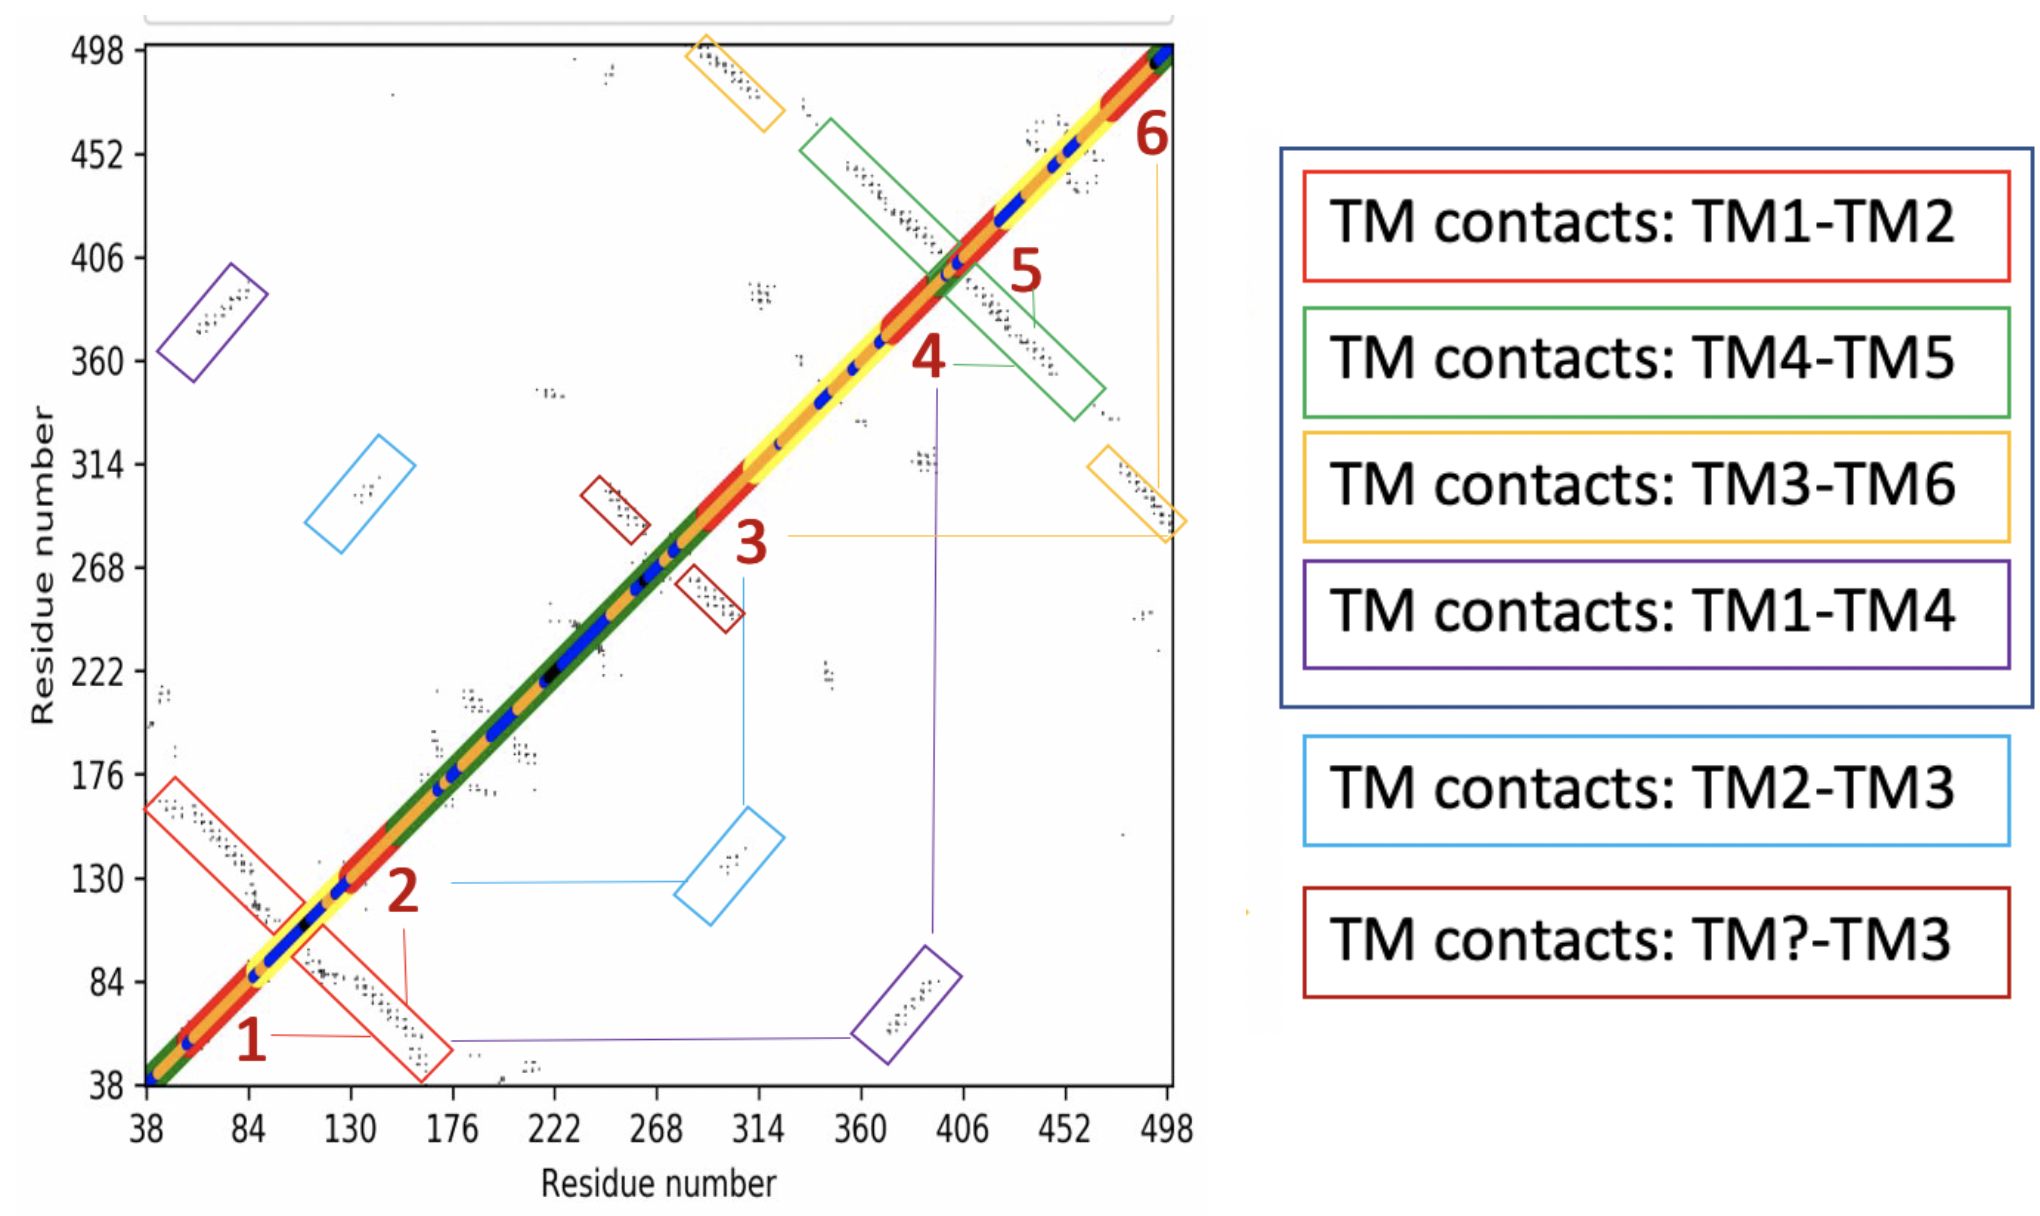
\includegraphics[width=\textwidth]{Modelling of Atg9/respred_cmap_anal.png}
    \caption{Atg9 ResPre TMD Contact map analysis}
    \label{fig:respr_anal}
    \small
    The Purple box groups predicted transmembrane helical contacts that are accounted for in the Lai et al (2020) paper.  Outside of the purple box are predicted transmembrane contacts that the Lai et al (2020) model does not account for. The coloured outlines of the boxes correspond to the positions of the contacts as annotated in the contact map.
\end{figure}
In order to evaluate the bioinformatic predictions provided in the paper a metagenomic enhanced ResPre contact map with the visualisation of embedded prediction data was constructed and used to compare with the helical contacts described in the Lai et al (2020) paper \ref{fig:respr_anal}.  The authors interpretation of their low-resolution map use predicted contacts between transmembrane 1 and 2, 4 and 5 , 3 and 6, and 1 and 4, all antiparallel. However, interpretation of the enhanced ResPre contact map strongly supports an orientation between TM1 and 4 as parallel. Also, the ResPre contact data shows a parallel signal between transmembrane 2 and 3. Both the parallel assignments 2-3 and 1-4 are inconsistent with the straightforward topology presented in the paper and suggests that the C- and N- termini are on opposing sides of the membrane rather than the same side (Figure \ref{fig:respre_anal2}).  This finding prompted a further investigation into the experimental origins of the accepted topology of Atg9 \cite{Young2006}. During the research by Young (2006) they obtained experimental data for the topology of the N- and C-terminal domains using in vitro translocation into microsomes, followed by protease protection. This was possible because they had specific antibodies to the N- and C-terminus. The experimental data supported a model of 6 transmembrane helices, with both termini in the cytosol.  However, the paper does highlight some property of the putative transmembrane between TM2 and 3 which was determined not to be a transmembrane:  Lai et al (2020) also highlight this in their paper from the homology of the plant protein with myosin proteins (Figure S6). This region is also of interest as it contains a large number of conserved residues. Additionally, the data in Young (2006) is more equivocal regarding the orientation of the C-terminus and not as robust as for the N-terminus. This all gives a basis for a possible alternative topology for Atg9.

\begin{figure}[th!]
    \centering
    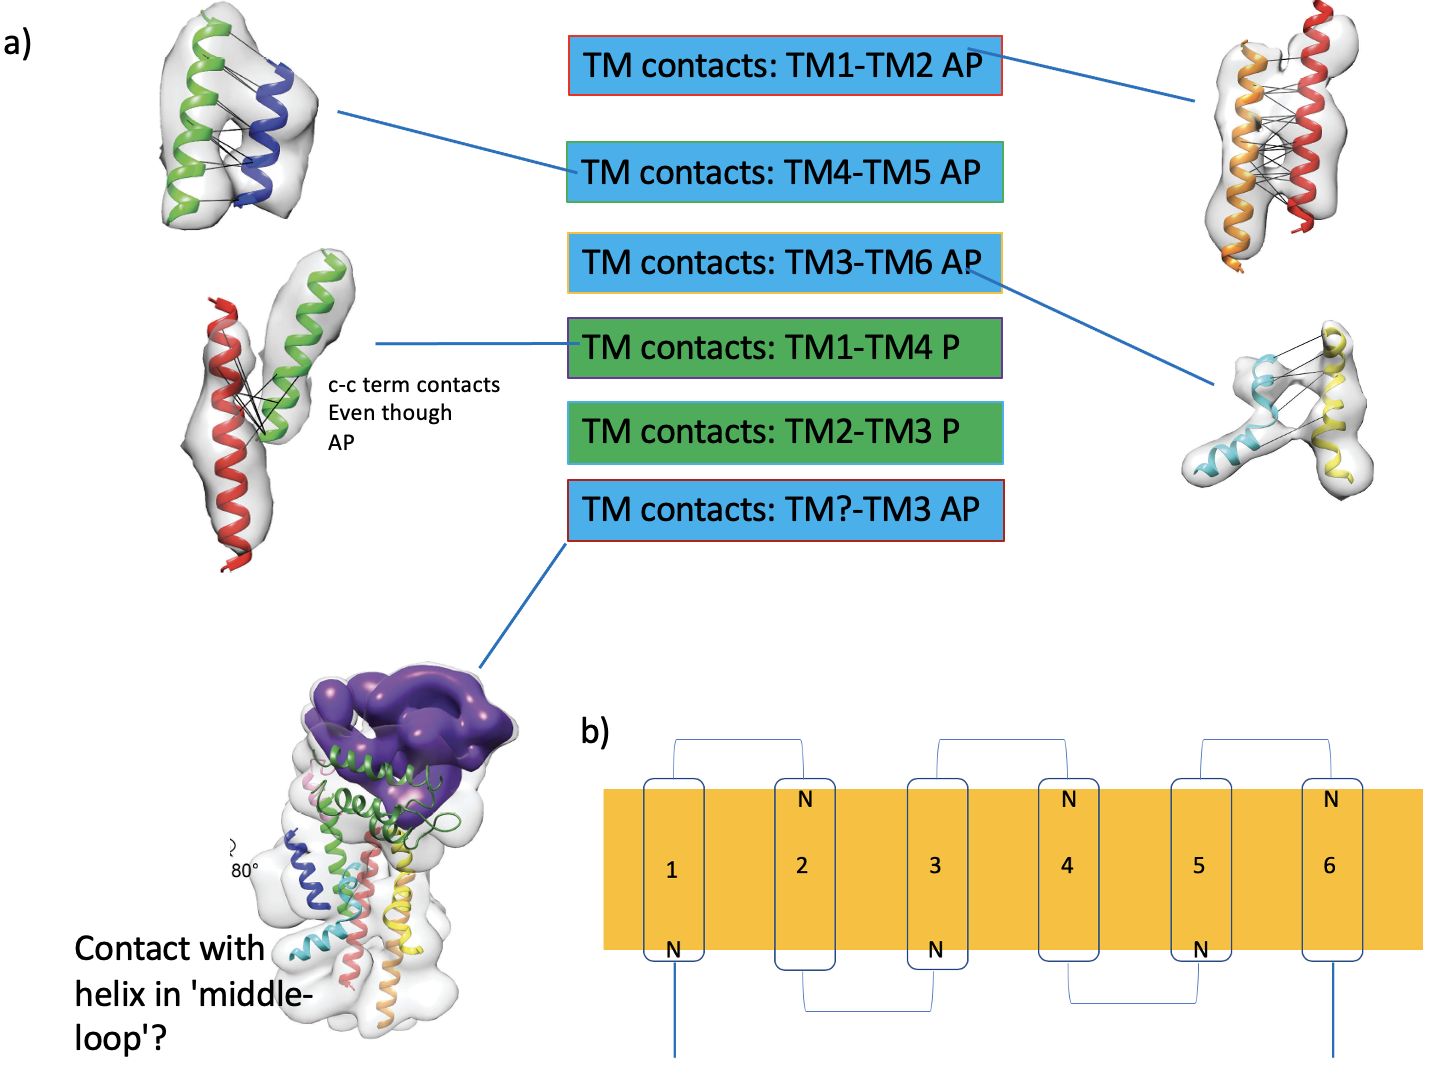
\includegraphics[width=\textwidth]{Modelling of Atg9/cmap_comparison_w_lai_etal.png}
    \caption{Comparison of Lai et al. low resolution interpretation with our contact data. }
    \label{fig:respre_anal2}
    \small
    a) Comparison of helical contacts with ResPre predicted helical contact features; blue boxes are helical contacts that are consistent with the proposed CryoEM model and green boxes are helical contacts that are inconsistent with the CryoEM model.  The coloured outlines of the boxes correspond to the positions of the contacts as annotated in \ref{fig:respr_anal} contact map. 'A' - parallel, 'AP' -  Anti-parallel.
    b) Established Atg9 topology.
\end{figure}

\newpage



\section{ABC Transporter Survey}
The strong co-variance data supports an alternative to the accepted topology for Atg9. The possible existence of an additional transmembrane helix between TM 2 and transmembrane 3 would satisfy the predicted contact map features. Submitting the putative transmembrane domain sequence of Atg9 to the transmembrane helix prediction tool TMHMM, does indeed show a weak signal for a predicted helix between transmembrane 2 and transmembrane 3 (Figure \ref{fig:atg9_tmhmm}). The presence of the weak TMHMM signal between predicted helices transmembrane 2 and 3 prompted an investigation into the possible
structural features that are responsible for these ‘blips’. As HHpred predicted a evolutionary link between Atg9 and ABC transporters, the sequences for experimentally solved ABC transporter structures were screened for the presence of these weak signals using TMHMM. The transmembrane domains of ABC transporters show low sequence conservation and are structurally divergent, with this diversity being related to their distinct functions. Screening the PDB (see specific methods) for ABC transporters resulted in 51 entries which can be classified into eight ABC transmembrane domain folds; Pgp, ABCG2, MalFG, BtuC, EcfT, LptFG, MacB, and MlaE \cite{srikant2020evolutionary}.  The sequences for each of the 51 entries were submitted to a local installation of TMHMM.  The TMHMM output results for each sequence were visually inspected. The screening identified ten ABC transporters with at least one weak transmembrane prediction TMHMM signal; 2ONK-C, 3WME-A, 4MRN-B, 4RYZ-A, 4TQV-A, 4TMS-C, 5DO7-A, 5MKK-B, 5NIK-J and 6AN7-D.  For each of these the TMHMM profile, predicted contact map and the crystal structure were visually cross referenced in order to identify any structural features that were the origin of the 'blip' being reported by TMHMM (Figure \ref{fig:3wme_tmhmm} shows one example - 3wme).  At the same time, contact features for the transmembrane domain of the predicted contact map were annotated to identify their representation on the actual crystal structure with the aim of cross referencing these with any common contact map features present in the Atg9 predicted contact map. 

\begin{figure}[htb]
\begin{subfigure}{0.3\textwidth}
  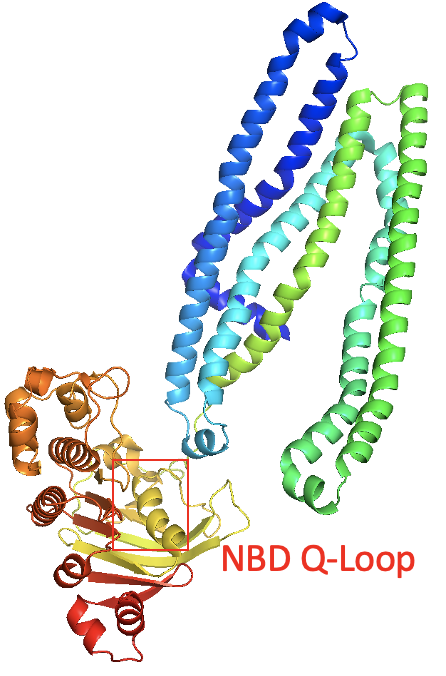
\includegraphics[width=\linewidth]{introduction/3wme.png}
  \caption{3wme Experimental Structure.  Colour spectrum, blue is N-terminal to red C-terminal.  Q-loop highlighted which corresponds to the position of TMHMM 'blip'.}
  \label{fig:0}
\end{subfigure}\hfil % <-- added
\begin{subfigure}{0.5\textwidth}
  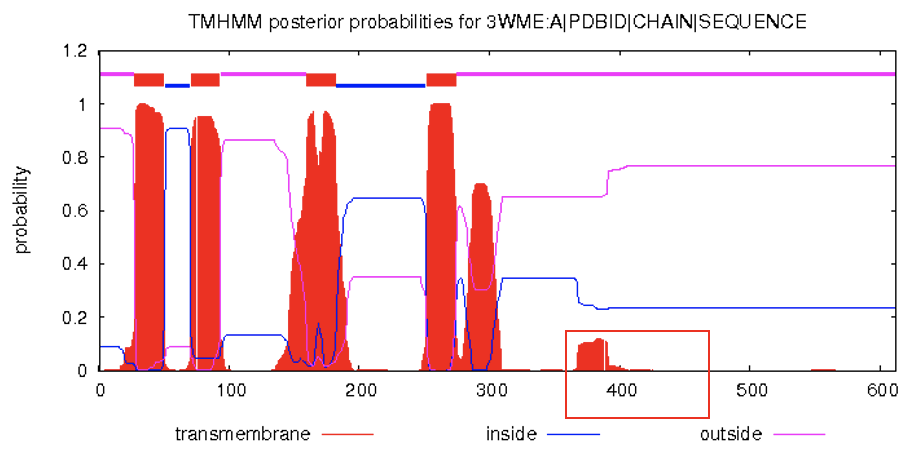
\includegraphics[width=\linewidth]{introduction/3wme_tmhmm.png}
  \caption{3wme TMHMM profile}
  \label{fig:atg9_tmhmm}
\end{subfigure}\hfil % <-- added
\caption{Analysis of 3wme TMHMM profile.  Red box highlighting 'blip'. }
\small
\label{fig:3wme_tmhmm}
\end{figure}

\begin{figure}[th!]
    \centering
    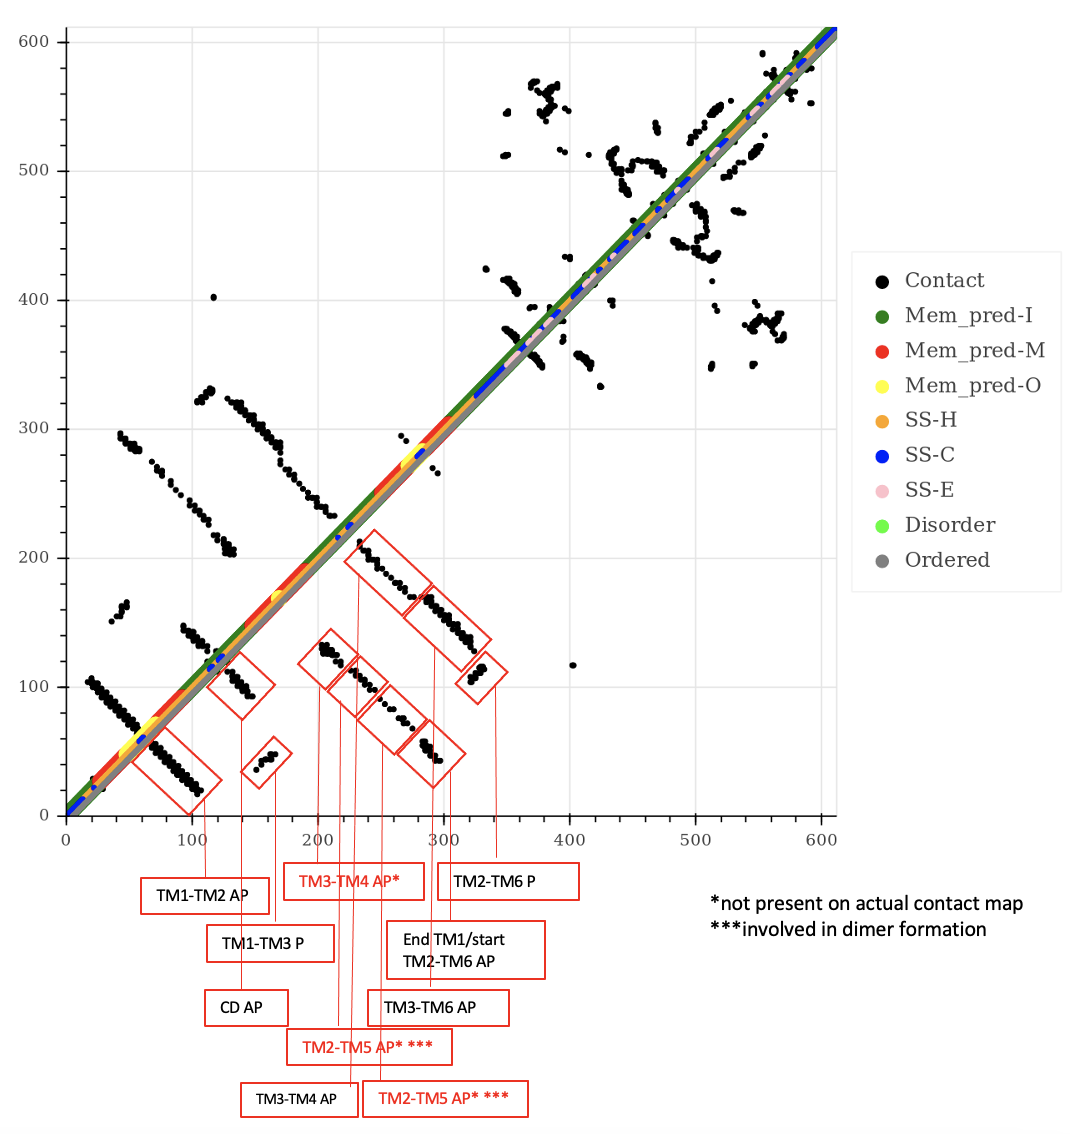
\includegraphics[width=100mm, scale=1]{introduction/3wme_cmap.png}
    \caption{3wme Predicted contact map analysis.    }
    \label{fig:3wme Contact map analysis}
    \small
    Transmembrane contact map features highlighted with red boxes.  Red font indicates contacts that are not present in the contact map of the experimental structure; black font indicates that features are shared by the contact map of the experimental structure. P-parallel, AP-antiparallel, I-inside, O-outside, M-membrane. 
\end{figure}

 The ABC transporter screen identified three features in ABC transporters that are responsible for a weak TMHMM transmembrane prediction signals; the nucleotide domain binding Q-loop, the extra-cellular domain and certain periplasmic helices (Figure \ref{fig:abc_tmhmm}); none of these structural features would be expected to be present in Atg9 due to the absence of the nucleotide binding domain. Also, such as in 4tqu (Figure \ref{fig:4tqu}),  a weak TMHMM was produced for a helix that has no specific function stated in the paper \cite{maruyama2015structure}. Additionally, there are cases such as in 4yms (Figure \ref{fig:4yms}) where the TMHMM prediction does not match the actual topology; five transmembrane helices are present in the crystal structure but only three were predicted.
 
 Analysing the predicted contact map features of the transmembrane domain of the ABC transporters in order to predict the structural feature representing the TMHMM 'blip' for Atg9 revealed that most of these features can be satisfied by the interhelical interfaces in the three dimensional structure when comparing to the contact map of the crystal.  There are examples, however, where the features are not satisfied by the structure; contacts responsible for dimer formation being present as well as  small contact features that cannot be satisfied by looking at the crystal structure and are possibly as a result of an alternative conformation (Figure \ref{fig:3wme Contact map analysis}).  In conclusion, the ABC transporter survey did not provide a firm indication as to what structural feature Atg9 possesses that would produce the TMHMM 'blip'.
 
 
\begin{figure}[htb]
\begin{subfigure}{0.25\textwidth}
  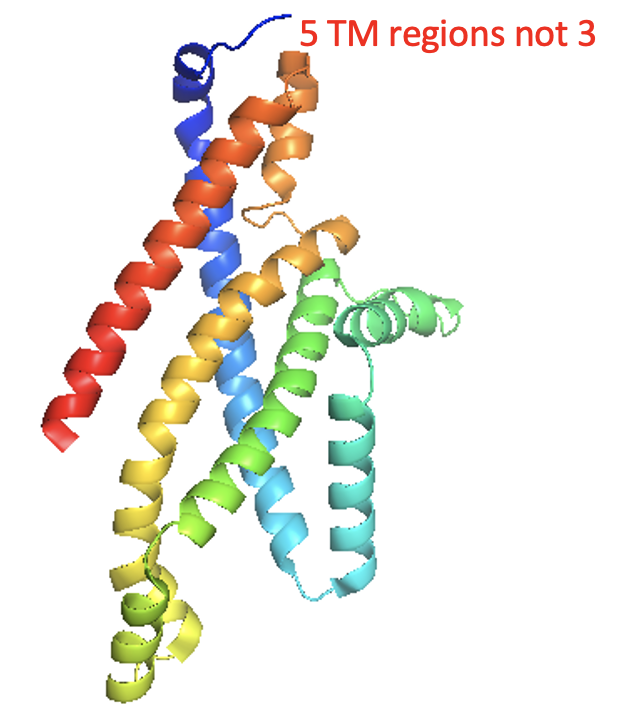
\includegraphics[width=\linewidth]{introduction/4yms.png}
  \caption{4yms}
  \label{fig:4yms}
\end{subfigure}\hfil % <-- added
\begin{subfigure}{0.25\textwidth}
  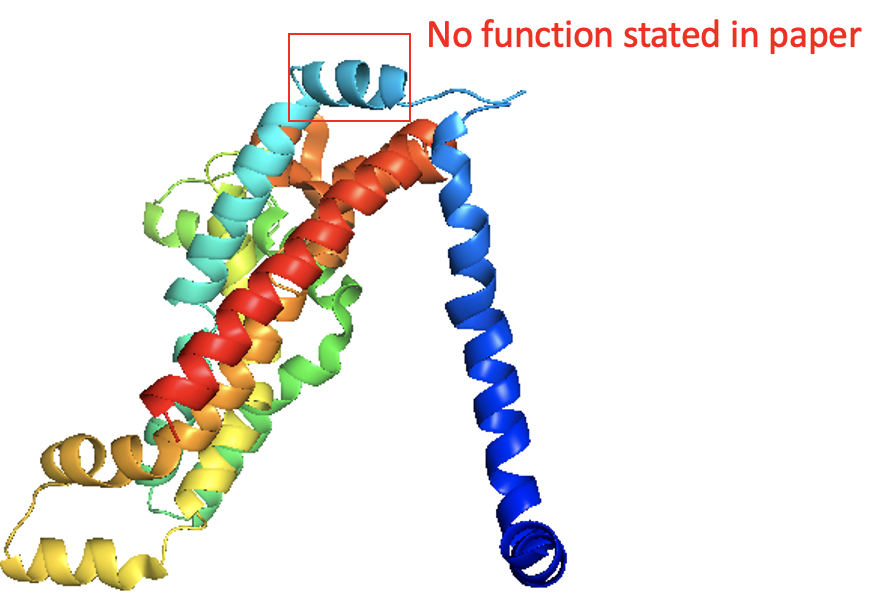
\includegraphics[width=\linewidth]{introduction/4tqu.png}
  \caption{4tqu}
  \label{fig:4tqu}
\end{subfigure}\hfil % <-- added
\begin{subfigure}{0.25\textwidth}
  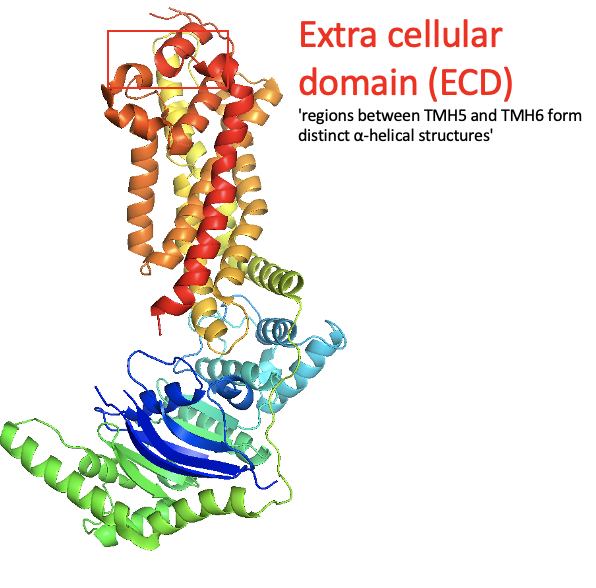
\includegraphics[width=\linewidth]{introduction/5do7.png}
  \caption{5do7}
  \label{fig:5do7}
\end{subfigure}\hfil % <-- added
\begin{subfigure}{0.25\textwidth}
  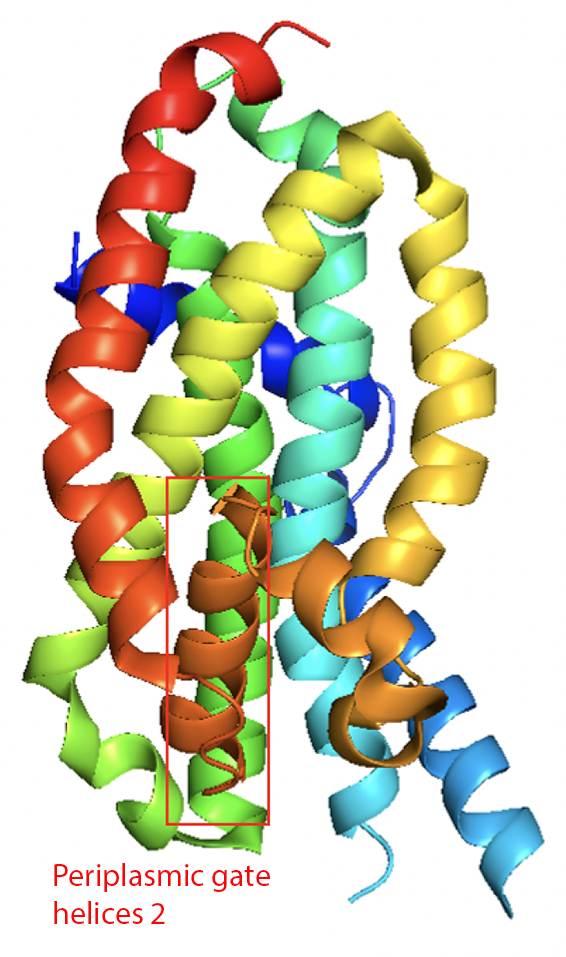
\includegraphics[width=\linewidth]{introduction/6an7.png}
  \caption{6an7}
  \label{fig:6an7}
\end{subfigure}\hfil % <-- added
\caption{Analysis of ABC TMHMM profiles by cross-referencing with experimental structures.}
\small
\label{fig:abc_tmhmm}
\end{figure}


\section{Analysis: High Resolution CryoEM Model}
\begin{figure}[th!]
    \centering
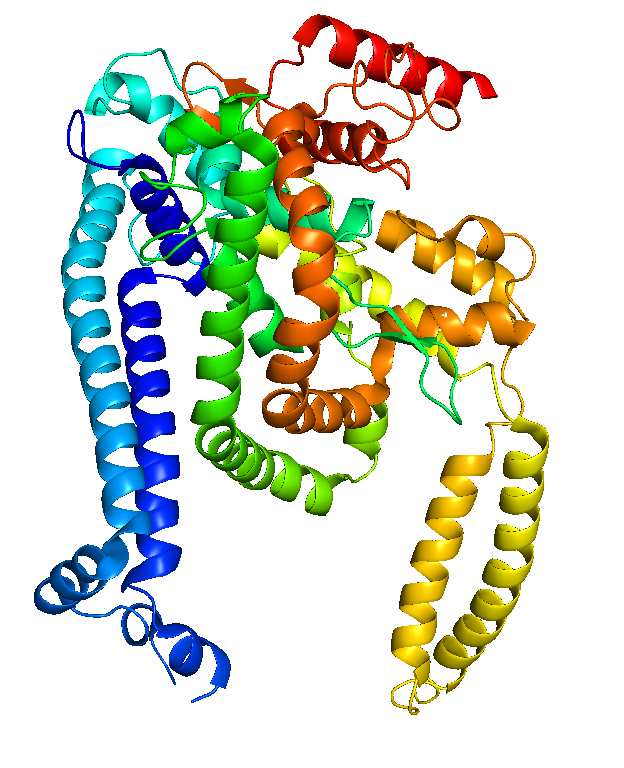
\includegraphics[width=\linewidth]{Modelling of Atg9/6wqz.png}
    \caption{Atg9 High resolution CryoEM model}
    \label{fig:6wqz}
    \small
    Atg9 monomer topology adapted from \cite{guardia2020structure}. Spectrum: Blue-N-terminal to red C-terminal.
\end{figure}

A second CryEM model of Atg9 was published (Figure \ref{fig:6wqz}) \cite{guardia2020structure} and in contrast to the previous published CryEM model it was high resolution at 2.9 Å.  The model revealed that Atg9 has a novel fold and is a domain-swapped homotrimer with the N- and C-terminal halves of the transmembrane domain being pseudo repeats;  consisting of two transmembrane helices and one re-entrant loop with sequence similarity identified locally around proline residues in the re-entrant loops.  The domain swapping involves  a domain of one of the subunits that extends into another subunit and interacts with the main domain of this subunit with this interaction being synonymic to that of the same domain in the monomer. In Atg9 two transmembrane helices from one monomer cross over and stack in parallel with two transmembrane helices from the neighboring monomer. The model also reveals an intricate system of cavities that are consistent with its putative role lipid in lipid transport.  Also molecular dynamics simulations predict that Atg9 has membrane-bending properties.

Comparing this high resolution accurate model to the bioinformatic work conducted for Atg9, the model did not support a six transmembrane helix topology for the transmembrane domain of Atg9.  The CryoEM model shows four transmembrane helices and two re-entrant loops. Transmembrane 1, 2, 4 and 5 (helices 2, 6, 14 and 15) were predicted correctly and transmembrane 3 and 6 (helices 11 and 19) were mis-classified and were actually revealed to be re-entrant loops.  The re-entrant loops present are atypical with the cytosolic N-terminal side extending out of the membrane by approximately 6 helical turns and a proline present at the membrane interface causing the helix to turn and run parallel before forming a loop and leaving the membrane on the same cytosolic side (Figure \ref{fig:atg9_pro}). 

\begin{figure}[th!]
    \centering
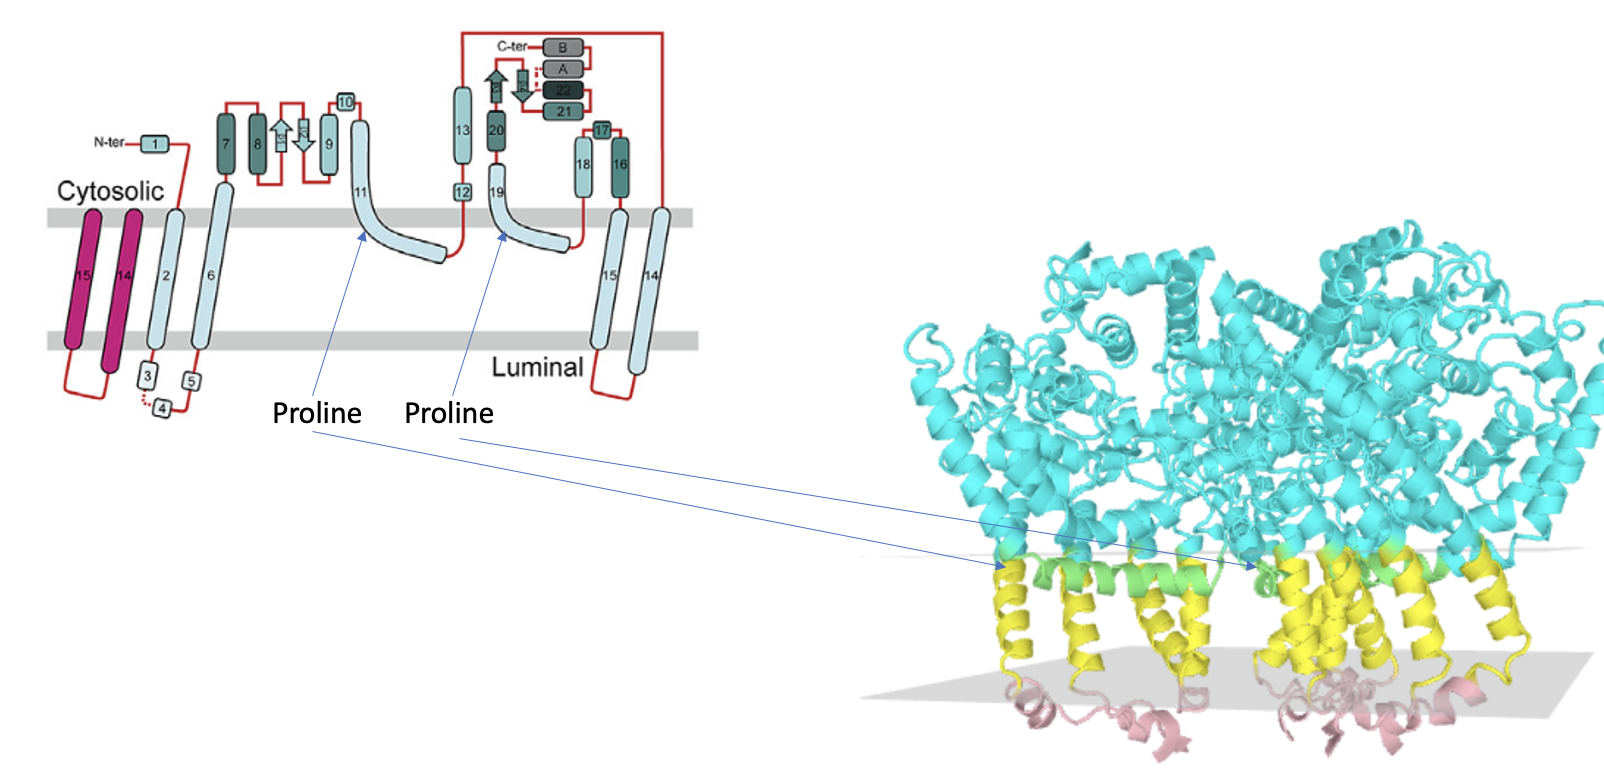
\includegraphics[width=\linewidth]{Modelling of Atg9/h_res_cro_anal2.png}
    \caption{Atg9 CryoEM Analysis}
    \label{fig:atg9_pro}
    \small
    Left: Atg9 monomer topology adapted from \cite{guardia2020structure}. Red helices are from and adjacent Atg9 forming the interface. Right: Atg9 trimer (blue are cytosolic regions, yellow are membrane embedded regions, pink are luminal regions and green are interfacial helical regions (boundaries for colouring and membrane planes obtained from the PDBTM \cite{Kozma2012}).
\end{figure}

In an effort to identify the mysterious 'blip' on the TMHMM prediction and the contact map features making contact with the 'blip', the relevant regions of the model were examined. The  TMHMM 'blip' was triggered by a short alpha helix (helix 9) on the cytosolic side of the membrane between transmembrane helix 1 and the first re-entrant loop.  The helix in question makes contact with the alpha helix that extends out of the membrane from the first N-terminal side of the first re-entrant loop (Figure \ref{fig:croem_anal1}).  Cross referencing transmembrane helical contacts in the cryoEM structure with the predicted contact map features of the transmembrane domain confirms that they are in agreement.

\begin{figure}[th!]
    \centering
    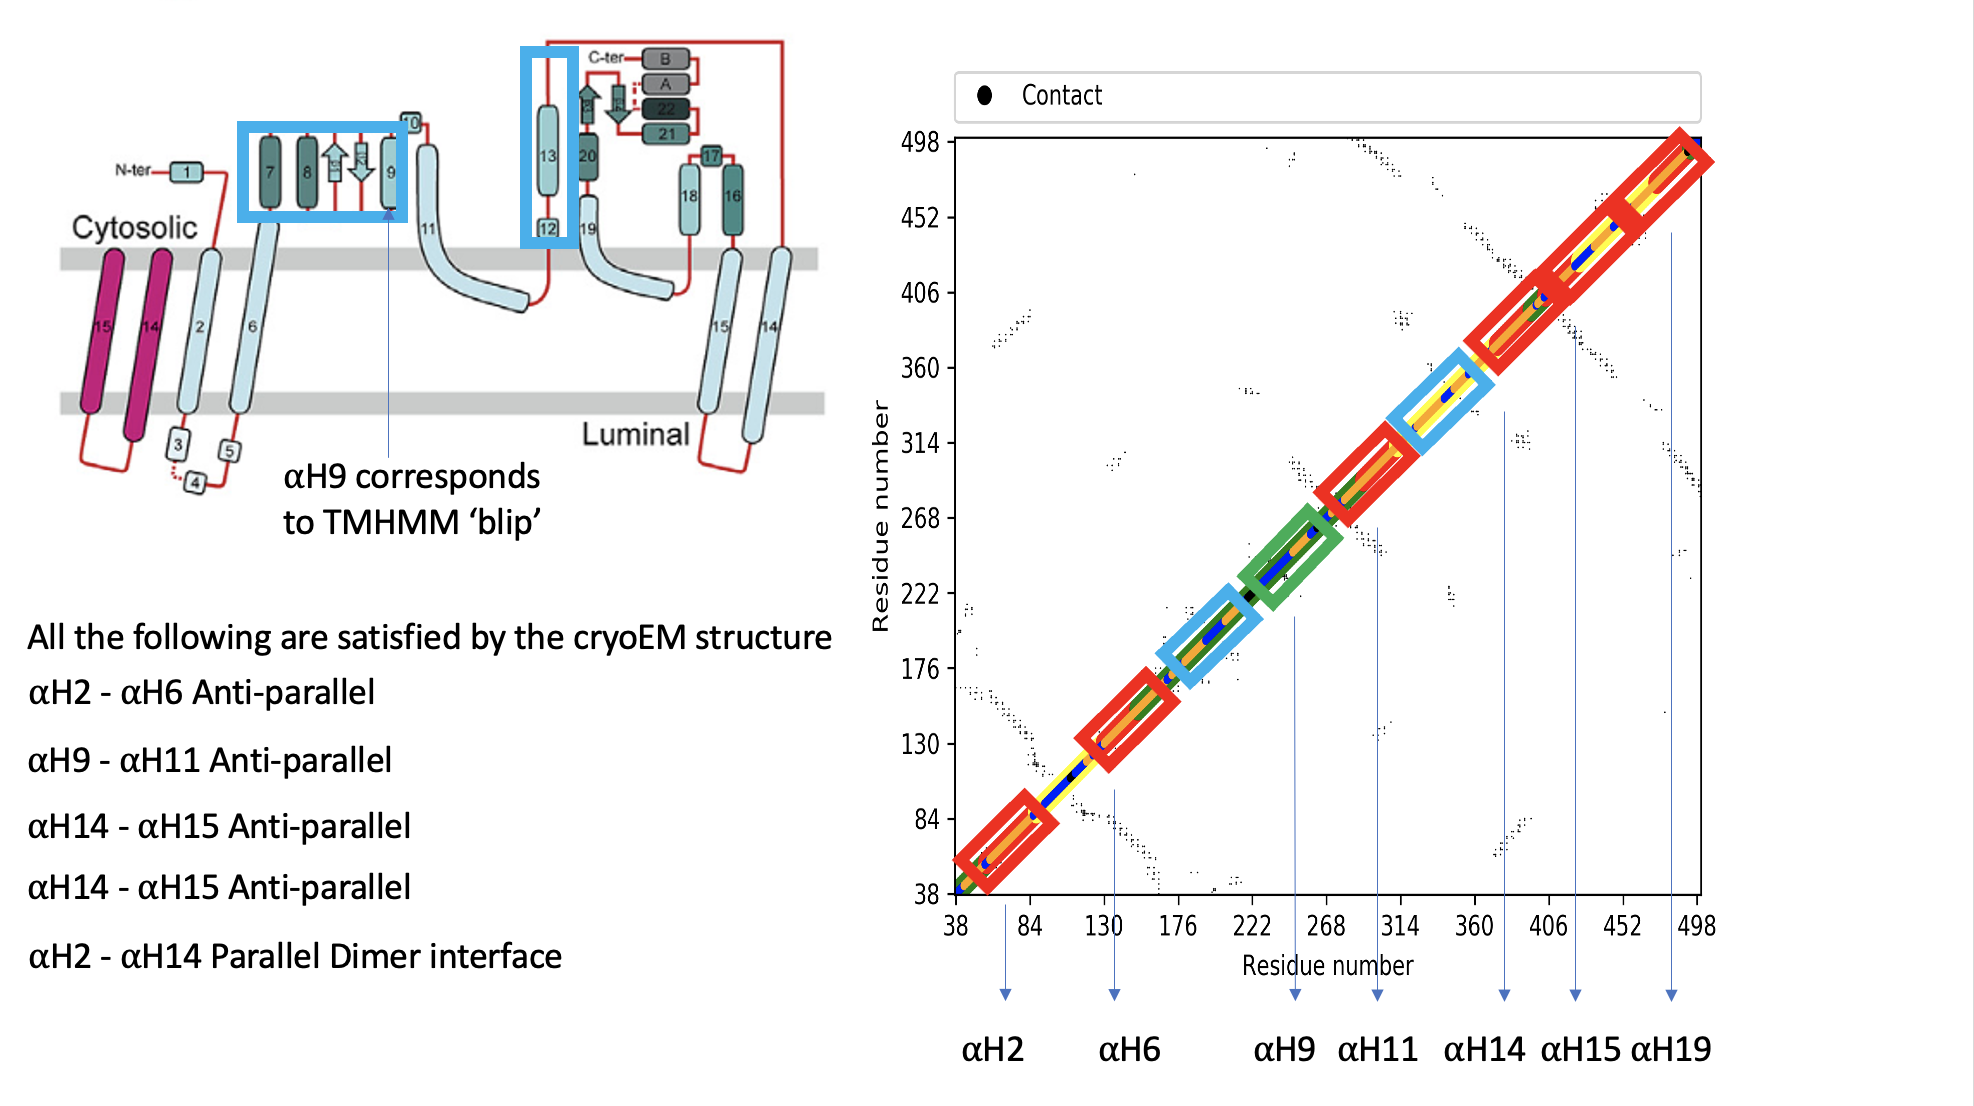
\includegraphics[width=\linewidth]{Modelling of Atg9/h_res_cro_anal1.png}
    \caption{Atg9 CryoEM Analysis}
    \label{fig:croem_anal1}
    \small
    Left: Atg9 monomer topology adapted from \cite{guardia2020structure}. Right: Respre predicted contact map for Atg9. Red boxes are regions of predicted transmembrane helices; green box is the region that contained the TMHMM 'blip'; blue boxes are regions of high sequence conservation.
    
\end{figure}

The successful CryoEM structure determination of Atg9 resulted in two models in alternate conformations.  An attempt to utilise contact predictions to indicate the plausibility of a third conformational state was carried out. The two contact maps from the alternate PDB conformation structures were compared to the predicted contact map in an effort to identify features that are present in the predicted map but not in the PDB files.  The presence of additional features might indicate that there is another conformational state as the predicted contact map will show superimposed contacts that are important from all conformational states. By subtracting away contacts explained by the known structures and getting any leftover plausible, consistent sets of strongly-predicted contacts would indicate further a biologically important conformation or, of course, contacts relating to oligomeric interfaces. Utilising ConKit the structural contacts sets of the two experimentally determined PDB structures were combined and mapped against the Atg9  predicted contact two-dimensional coordinates (Figure \ref{fig:atg9_conformation}). The Figure \ref{fig:4.16a} contact map on the left shows grey points representing the predicted contacts for Atg9, black points are the predicted contacts satisfied by structural contacts and red points are contacts present in the structure but not present in the predictions.  Three predicted contact features (pink, yellow and blue boxes) in the same area of the contact map (green) not present in the structures were identified. The corresponding regions were mapped on to Atg9 (right).  In the monomer these contacts could not be explained. Figure \ref{fig:4.16b} shows unsatisfied contacting regions from the predicted contacts mapped on to the trimer; the trimeric state accounts for the three sets of contacts not satisfied by the monomer.

\begin{figure}[htb]
    \centering % <-- added
\begin{subfigure}{0.75\textwidth}
  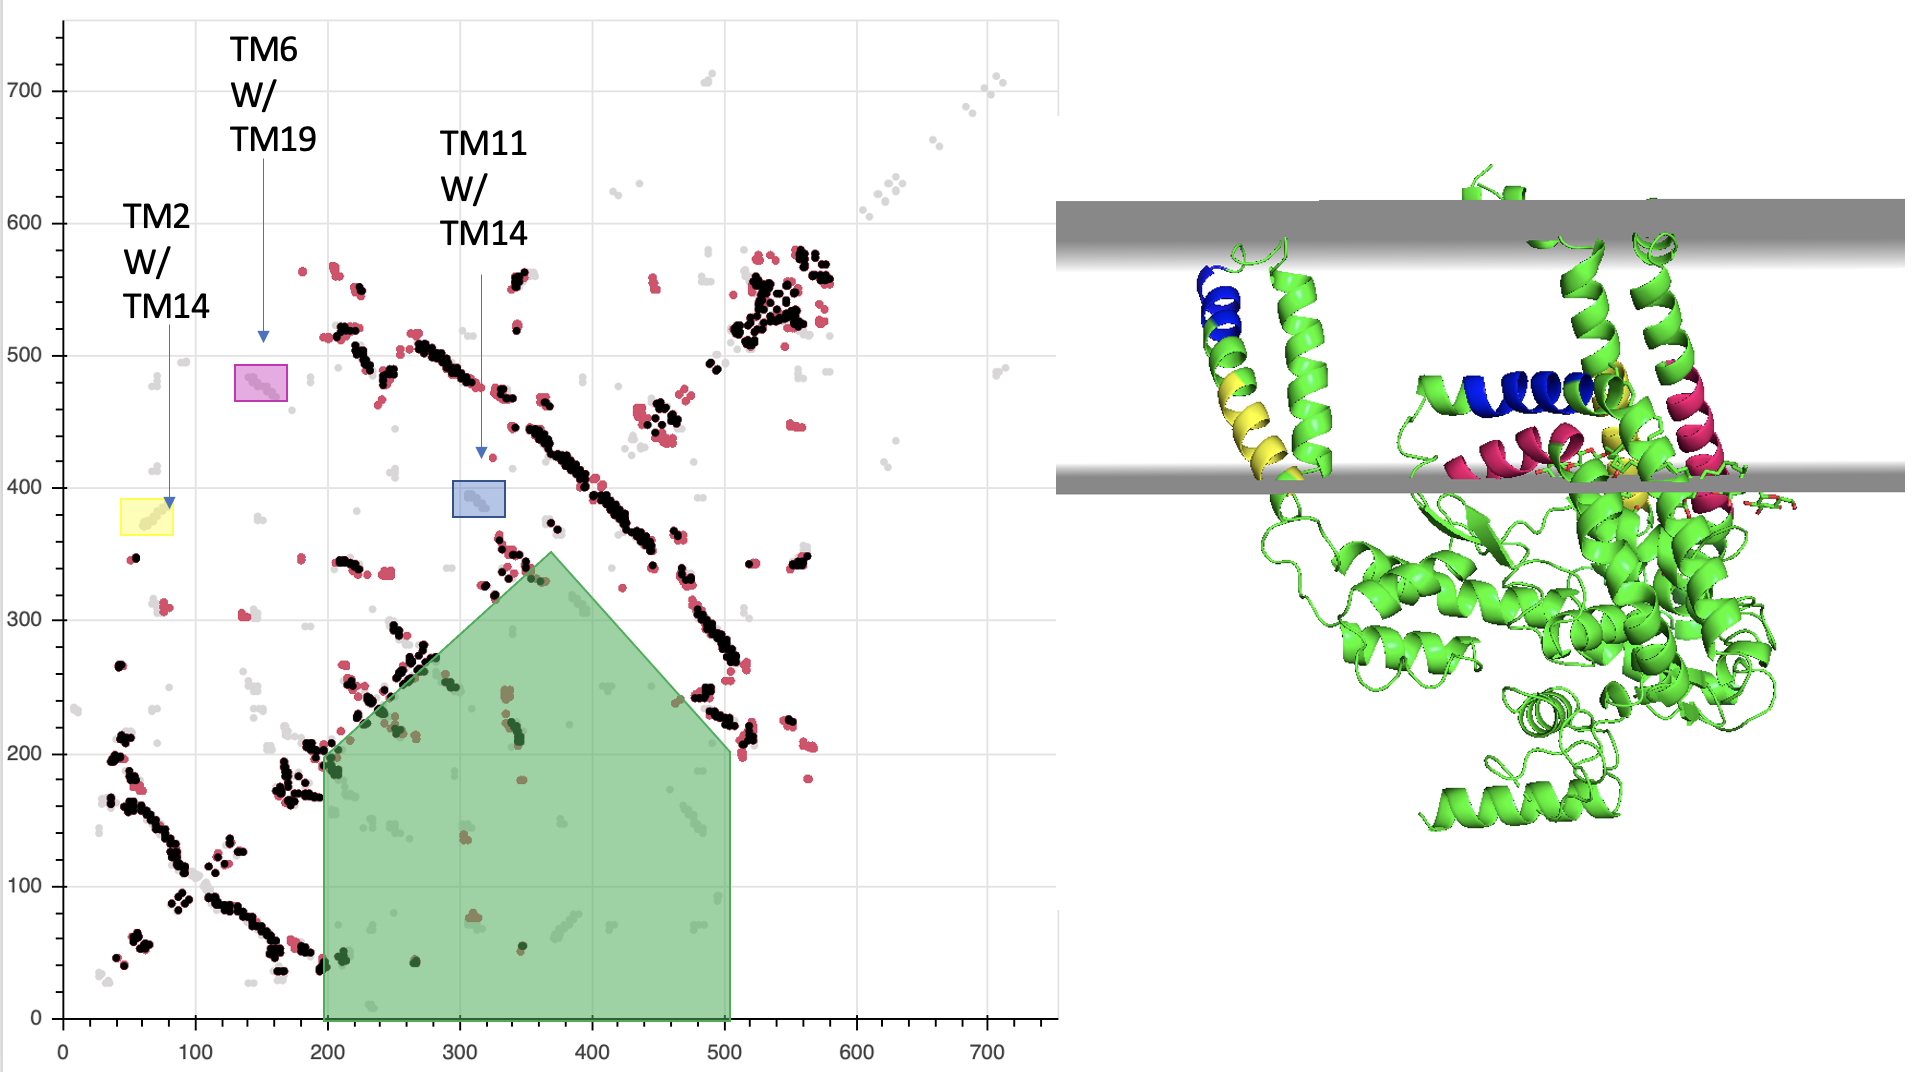
\includegraphics[width=95mm, scale=0.9]{introduction/cryo_cmap_anal.png}
  \caption{Superposition of CryoEM contacts for both conformations with predicted contact maps comparison.  Green shaded area indicates transmembrane region where unaccounted contacts are present. Corresponding colours of boxes on the contact map (left) are mapped on to the Atg9 monomer (right) (these shaded regions mirrored across the diagonal).  In the monomer these contacts cannot be explained.}
  \label{fig:4.16a}
\end{subfigure}\hfil % <-- added
\begin{subfigure}{0.75\textwidth}
  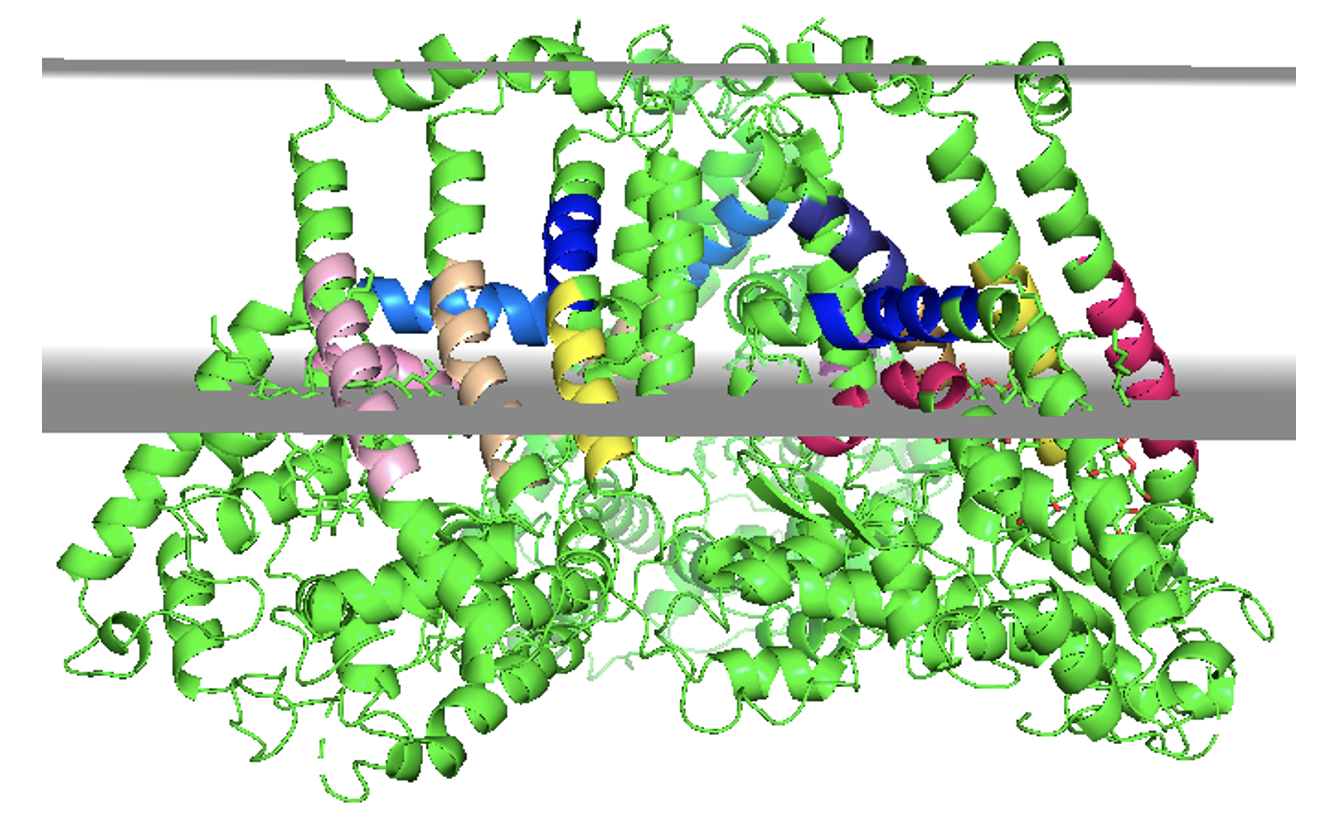
\includegraphics[width=85mm, scale=0.9]{introduction/cryo_cmap_anal2.png}
  \caption{Inter-chain contacts. Corresponding colours of boxes on contact map (left Figure \ref{fig:4.16a}) are mapped on to the Atg9 trimer.The trimeric state accounts for the three sets of contacts not satisfied by the monomer}
  \label{fig:4.16b}
  \small
  
\end{subfigure}\hfil % <-- added
\caption{Atg9 CryoEM Contact Analysis}
\small

\label{fig:atg9_conformation}
\end{figure}

Unfortunately, the evolutionary co-variance data did not provide any evidence for a third conformation. The predicted contact map of Atg9 is a superposition of inter- and intra-chain contacts. The PDB files contain the actual inter and intra chain contacts. The contact predictions for Atg9 were all satisfied by the actual contacts from the two Atg9 CryEM structures. Therefore, based on co-variance analysis there were no additional contacts that would be required to suggest an additional conformation.  However, examining the contact prediction map it can be seen that there are very few contact predictions for the residues after position 600. Visualising the actual contacts for 6wr4 it is true that there are few contacts for residues 600 onward, however, for the 6wqz conformation there are obviously contacts present that were never predicted.  Indeed examining the sequence coverage for both the Uniprot and metagenomic MSAs used for the co-variance analysis to construct the contact predictions for Atg9, figure \ref{fig:atg9_msa} reveals that after residue 600 there is poor sequence coverage.  The poor sequence coverage for residues after 600 indicates that there is not enough data to perform co-variance analysis here and to make contact predictions for the C-terminal end of Atg9. Therefore, the limitations in data quality mean that a third conformation cannot be ruled out.

In terms of a predicted function or a predicted characterisation of a substrate for this putative transporter further analysis was unable to determine any plausible possibilities. Conservation was mapped on to the PDB structures and regions of high conservation were visualised. The region between helix 7 and 9 along with helix 13 and 12 is highly conserved and therefore critical to structure or function (Figure \ref{fig:croem_anal1}). 

\section{Potential homology between the Atg9 and ABC transporters}

 The availability of a high resolution model gave rise to the opportunity to further examine the possibility of obtaining structural evidence to support the HHpred determined sequence similarity to Type I ABC transporters.  An attempted DALI pairwise structural alignment could not align the top HHpred PDB hit Type I ABC transporter 5w81 with Atg9.  Subsequently both structures were visualised in PyMol and the regions corresponding to HHpred alignment on both structures were highlighted (Figure \ref{fig:croem_vs_5w81}).


\begin{figure}[th!]
    \centering
    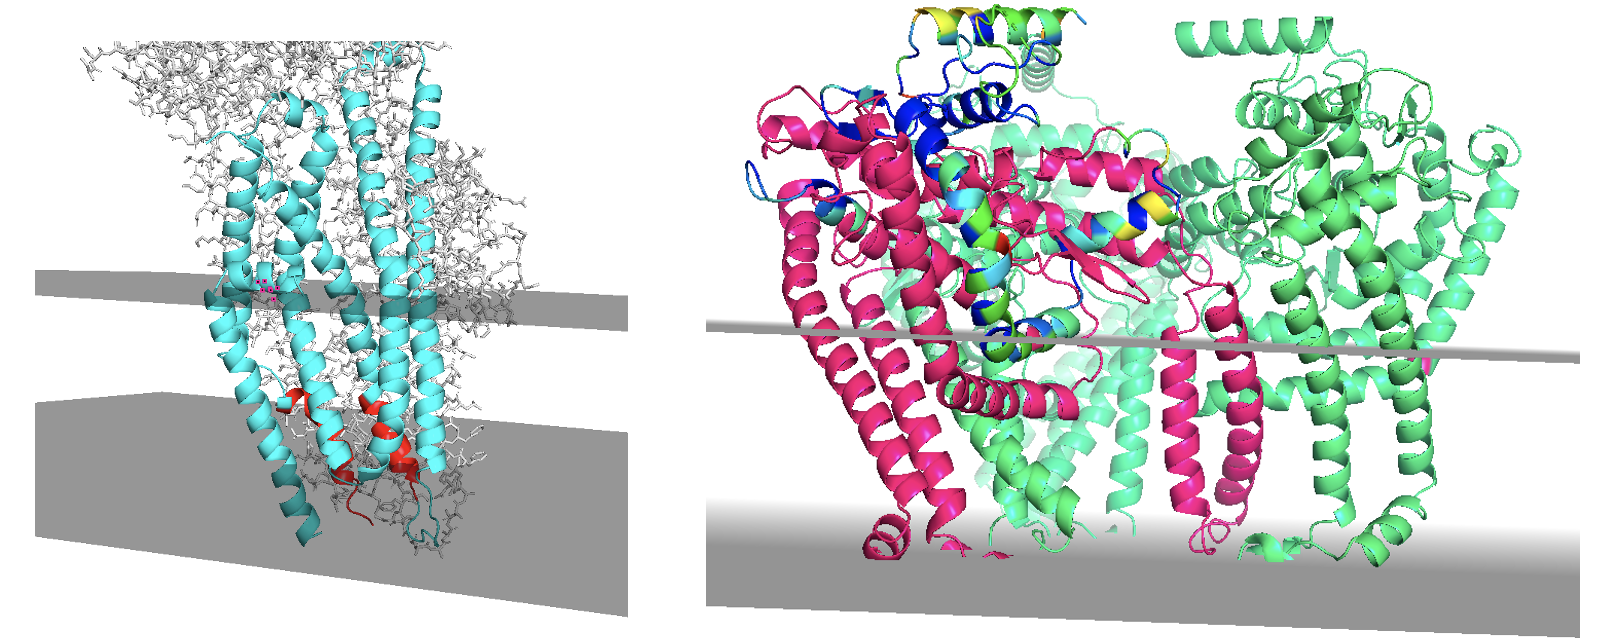
\includegraphics[width=\linewidth]{Modelling of Atg9/cryo_vs_5w81.png}
    \caption{Atg9 CryoEM comparison to 5w81}
    \label{fig:croem_vs_5w81}
    \small
    Cyan (on left image): regions of alignment of 5w81 with Atg9 (ribbon, non-aligned regions shown as wire); Pink (on right image):regions of alignment of Atg9 with 5w81; Green: non-aligned regions; Blue are highly conserved non aligned regions. 
\end{figure}

Assuming that Atg9 and Type 1 ABC transporters are distant homologues, comparing the topologies of the highlighted regions on both models show that the internal repeat unit of Atg9 is similar to the to the region between transmembrane 1 to transmembrane 3 in the ABC transporter;   transmembrane 3 of the ABC transporter is not a re-entrant loop (Figure \ref{fig:abc_topo}) and the re-entrant loop has straightened forming a transmembrane helix or alternatively one half of the transmembrane helix has developed a major kink forming forming the unusual Atg9 re-entrant loop.  A similar observation of evolutionary modification of transporter helices has been shown previously in CPA/AT transporters \cite{sudha2021evolutionary}.

\begin{figure}[th!]
    \centering
    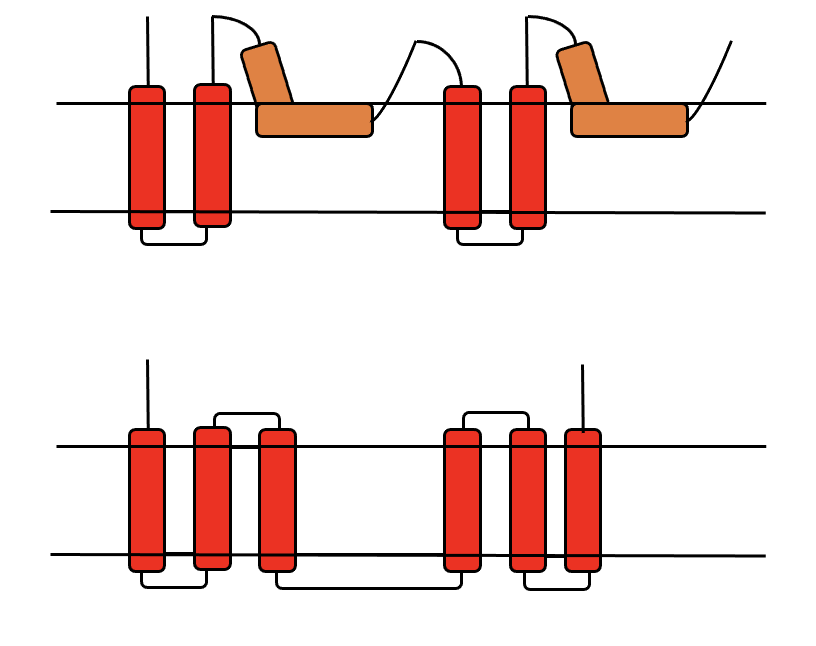
\includegraphics[width=100mm, scale=0.9]{Modelling of Atg9/atg9_topo_abc.png}
    \caption{Comparison of Atg9 and 5w81 topology}
    \label{fig:abc_topo}
    \small
    Top: Transmembrane domain topology of Atg9; Bottom: Transmembrane domain topology of typical Type 1 ABC transporter.
\end{figure}

This structural observation is reinforced by performing a PDB search using HHpred for the first repeat unit of Atg9 (residues 1-300). HHpred reported top scores of 20\%-45\% probability matches with the N- terminal region of the transmembrane domains of various Type I ABC exporters.  The first two N-terminal transmembrane helices of the ABC transporters aligned with the two N-terminal transmembrane helices of Atg9. The third transmembrane helix of the ABC transporter, however, did not align with the N-terminal re-entrant loop; this could be because of a difficulty to broaden the alignment due to the long insertion between transmembrane helix 2 and the first re-entrant loop in Atg9.

The sequence and structural evidence supporting an evolutionary link between Atg9 and Type I ABC transporters has recently been reported by another group \cite{maeda2020structure} who additionally superimposed the Type I ABC transporter, MsbA, bound to its substrate LPS with the C-terminal half of Atg9; interestingly this places LPS in a similar position to lipids bound to Atg9 \cite{maeda2019autophagic}. 

\section{Use of Deep Learning Methods}

Modelling of Atg9 using traditional fragment based assembly methods, even with meatagenomic derived contact information, was always going to be difficult due to the immense conformational space resulting from Atg9 being a large protein.  The release of newer modelling methods utilising distances and side-chain orientations such as DMPfold (Figure \ref{fig:4dmp_m1} and Figure \ref{fig:4dmp_m2}) also struggled with Atg9 modelling where contact satisfaction profiles were poor when compared against the high resolution Atg9 CryoEM model (Figure \ref{fig:atg9_dmp_m1_quality} and Figure \ref{fig:atg9_dmp_m2_quality}).  This difficulty in modelling could be related to the fact that Atg9 possesses a novel fold therefore the trained neural networks would have difficulty in constructing a model for a new fold.




\begin{figure}[th!]
    \centering
    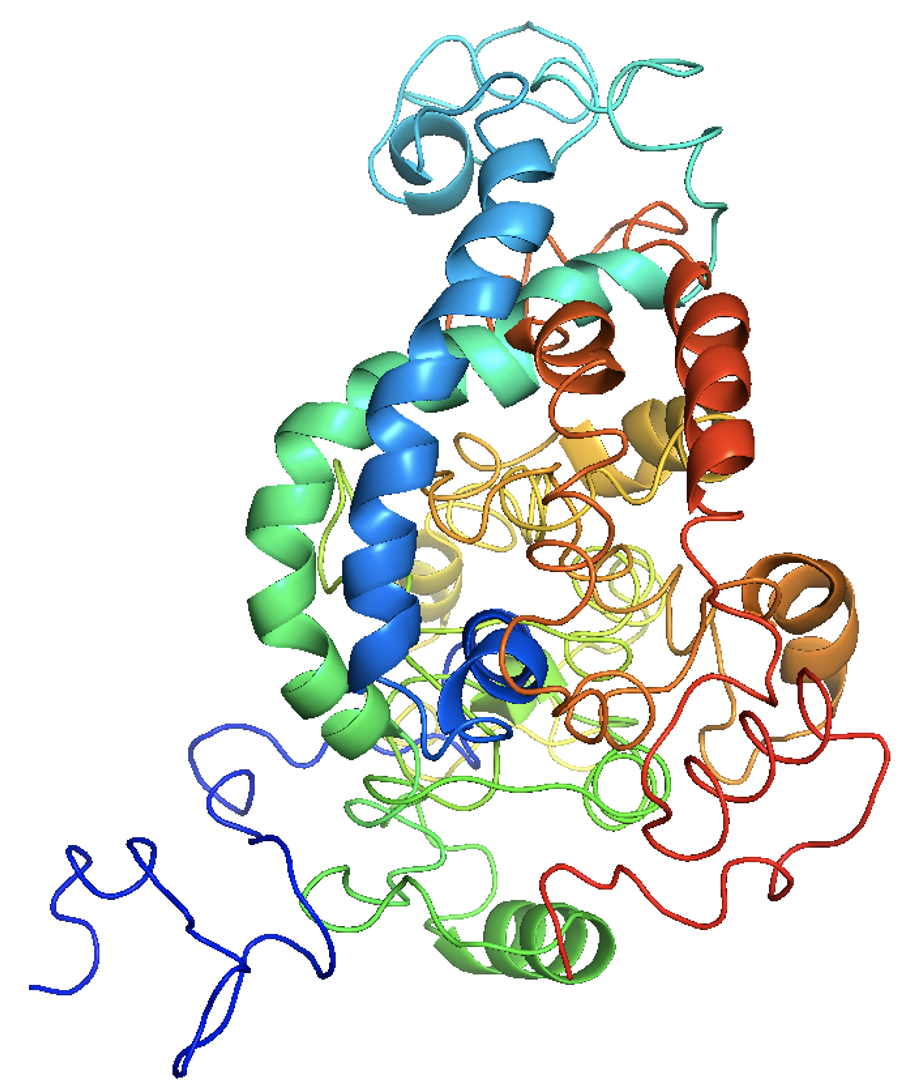
\includegraphics[width=50mm, scale=0.5]{Modelling of Atg9/dmp_m1.png}
    \caption{Atg9 TMD DMPFold Model 1}
    \label{fig:4dmp_m1}
    \small
\end{figure}

\begin{figure}[htb]
    \centering % <-- added
\begin{subfigure}{0.25\textwidth}
  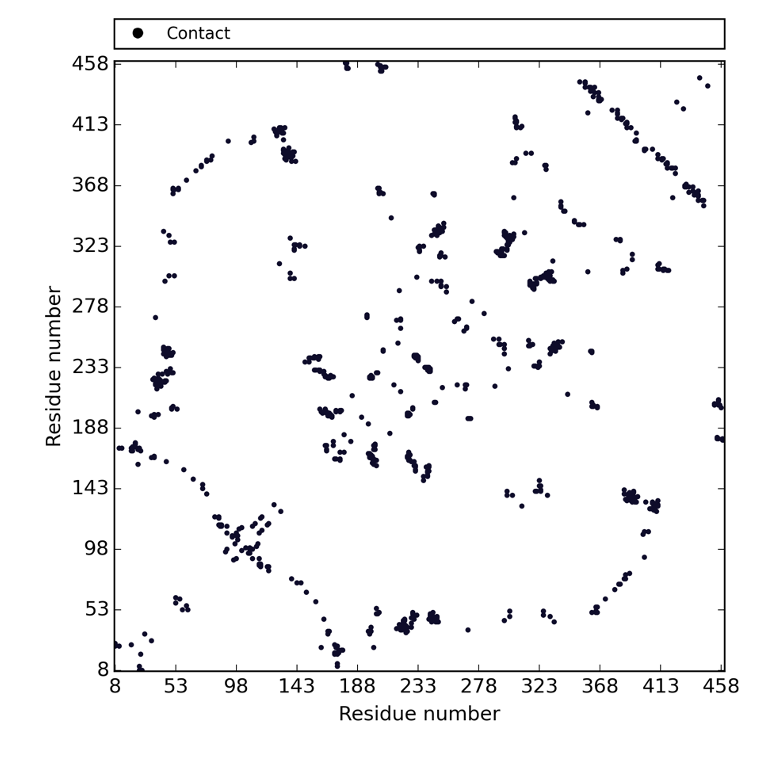
\includegraphics[width=\linewidth]{Modelling of Atg9/dmp_m1_cmap.png}
  \caption{Contact Map for DMPFold Model 1}
  \label{fig:0}
\end{subfigure}\hfil % <-- added
\begin{subfigure}{0.25\textwidth}
  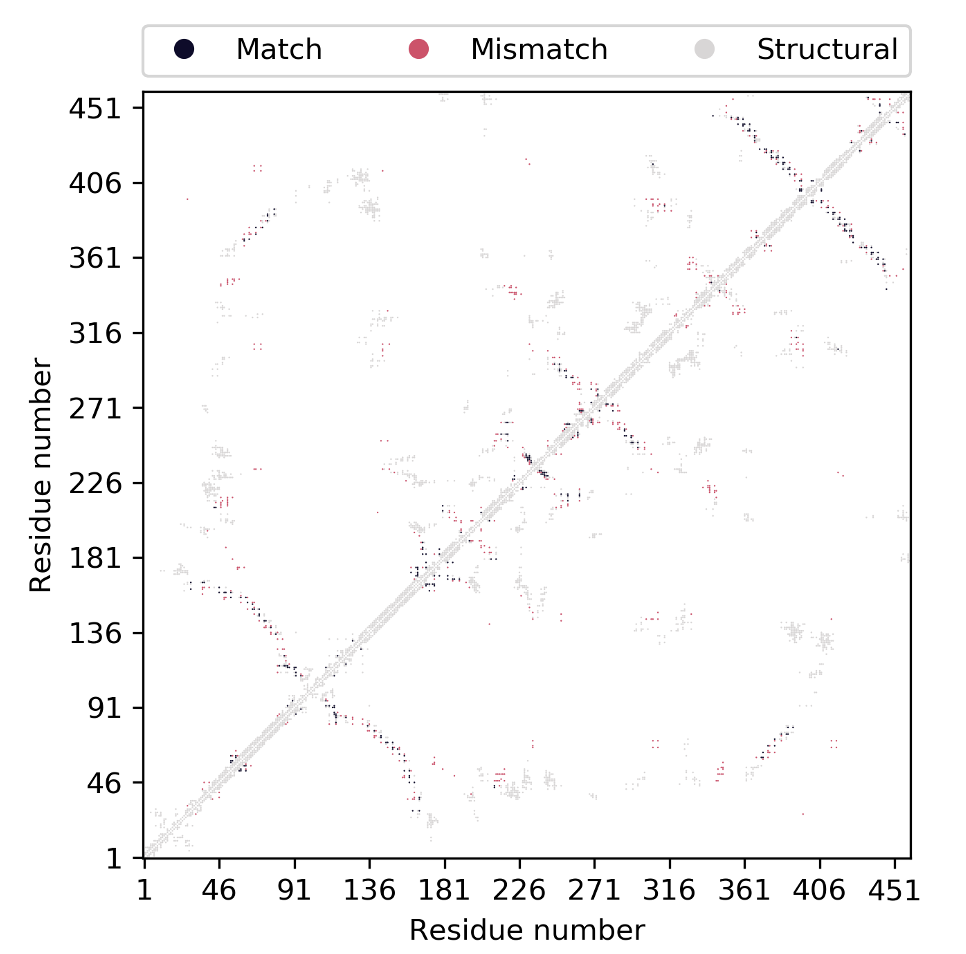
\includegraphics[width=\linewidth]{Modelling of Atg9/dmp_m1_super.png}
  \caption{Superposition of Atg9 DMPFold Model 1 Contact Map with the High Resolution Atg9 CryoEM contact map}
  \label{fig:1}
\end{subfigure}\hfil % <-- added
\begin{subfigure}{0.25\textwidth}
  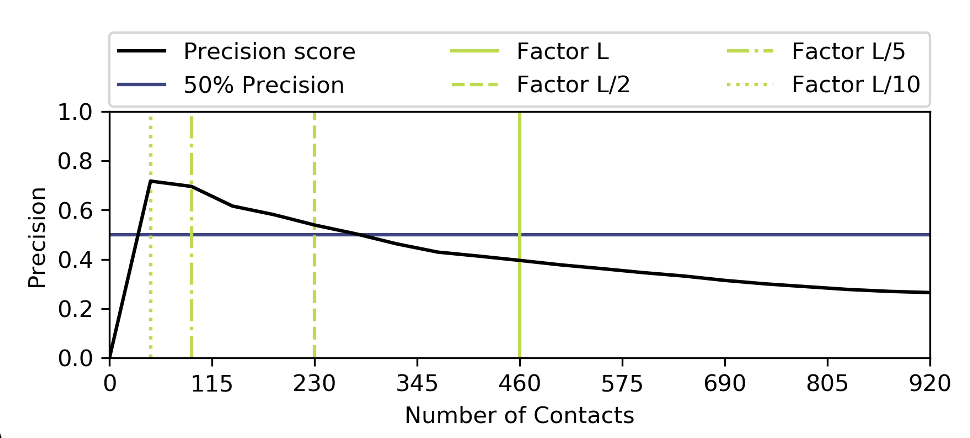
\includegraphics[width=\linewidth]{Modelling of Atg9/prec_dmp_m1.png}
  \caption{Precision profile of the Atg9 DMPFold model 1 against High Resolution Atg9 CryoEM Contacts}
  \label{fig:1}
\end{subfigure}\hfil % <-- added
\caption{Atg9 DMPFold Model 1 Quality Determination}
\small
\label{fig:atg9_dmp_m1_quality}
\end{figure}

\begin{figure}[th!]
    \centering
    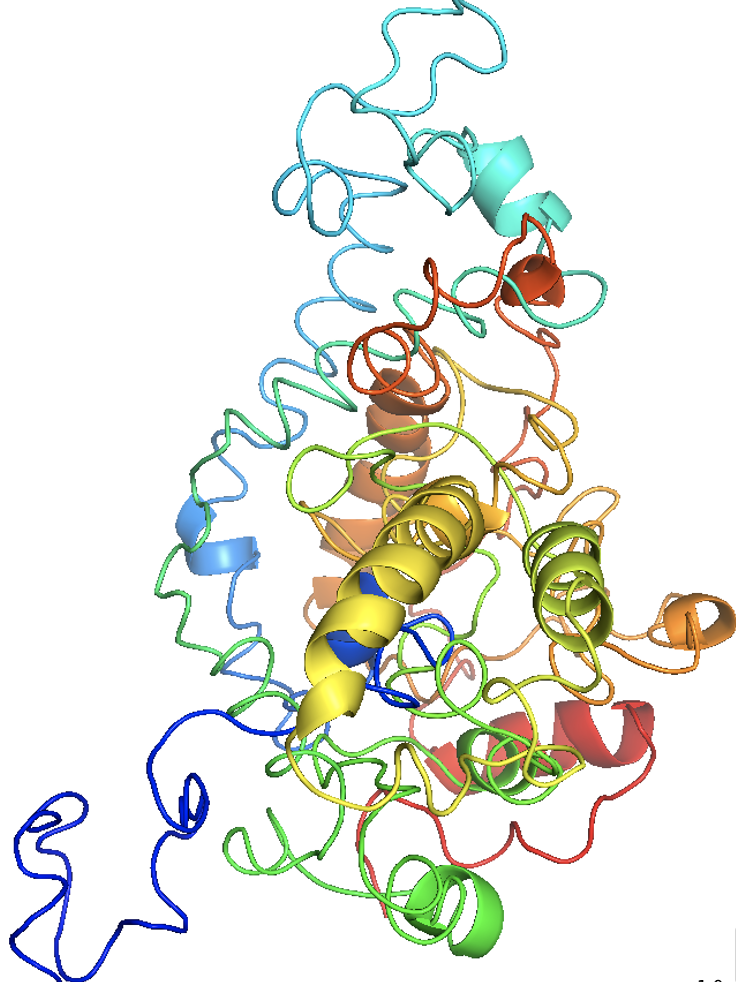
\includegraphics[width=50mm, scale=0.5]{Modelling of Atg9/dmp_m2.png}
    \caption{Atg9 TMD DMPFold Model 2}
    \label{fig:4dmp_m2}
    \small
\end{figure}

\begin{figure}[htb]
    \centering % <-- added
\begin{subfigure}{0.25\textwidth}
  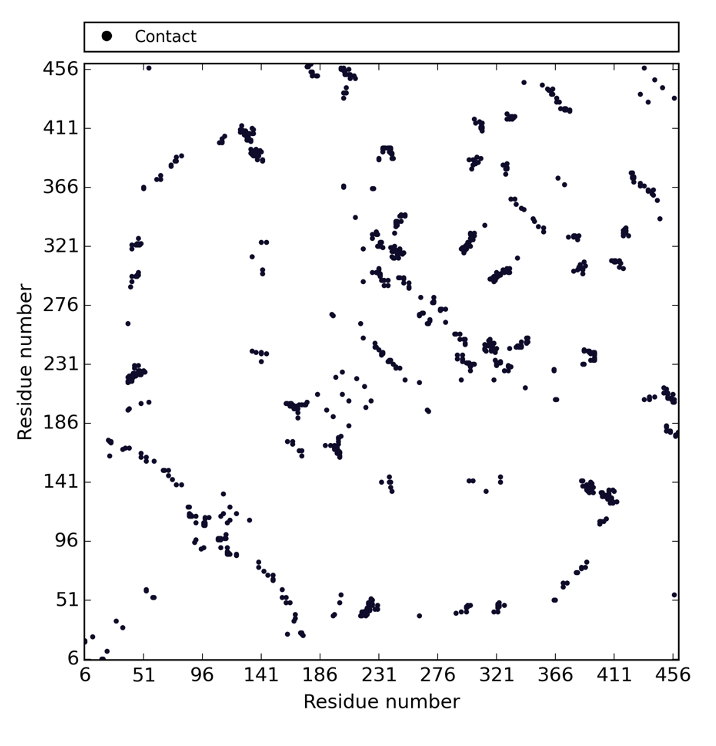
\includegraphics[width=\linewidth]{Modelling of Atg9/dmp_m2_cmap.png}
  \caption{Contact Map for DMPFold Model 2}
  \label{fig:0}
\end{subfigure}\hfil % <-- added
\begin{subfigure}{0.25\textwidth}
  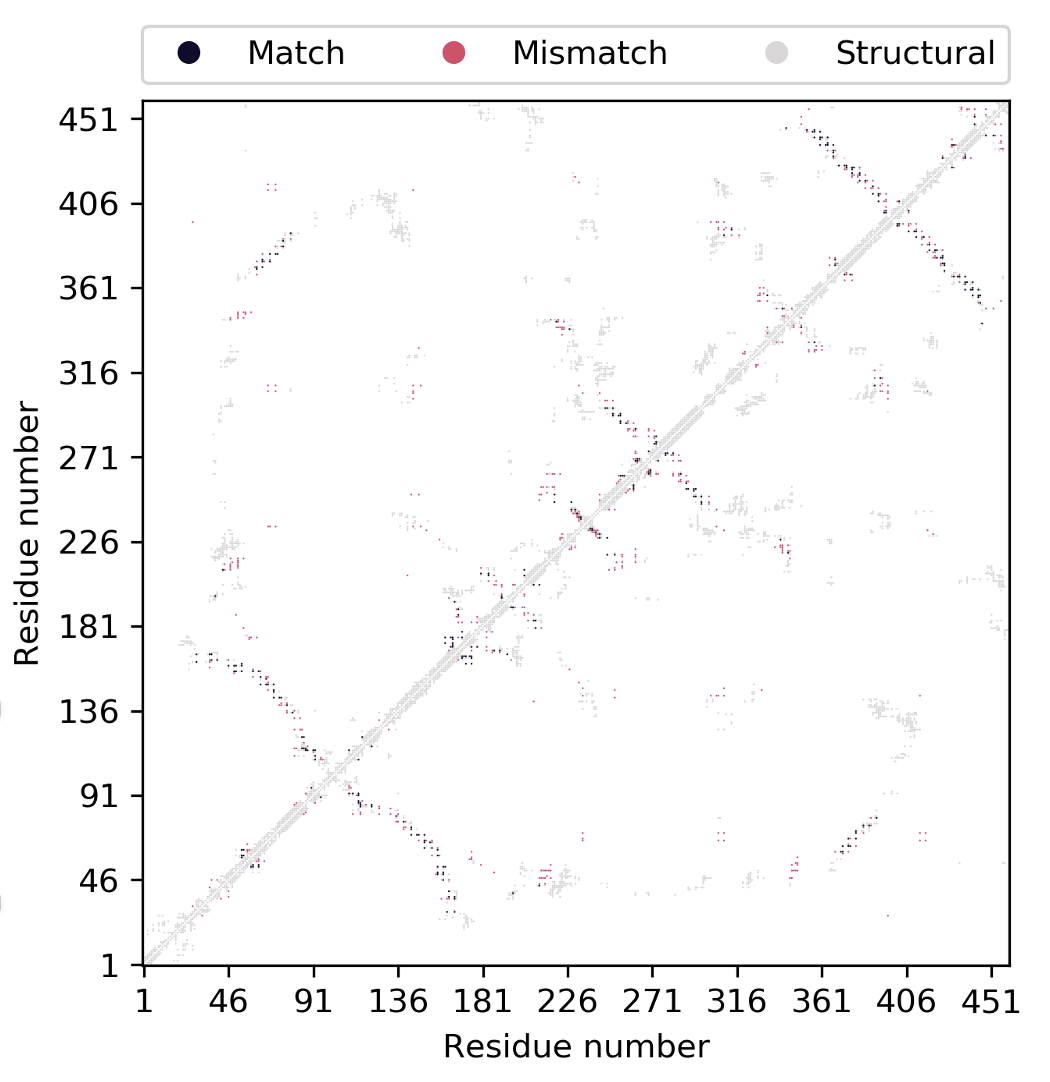
\includegraphics[width=\linewidth]{Modelling of Atg9/dmp_m2_super.png}
  \caption{Superposition of Atg9 DMPFold Model 2 Contact Map with the High Resolution Atg9 CryoEM contact map}
  \label{fig:1}
\end{subfigure}\hfil % <-- added
\begin{subfigure}{0.25\textwidth}
  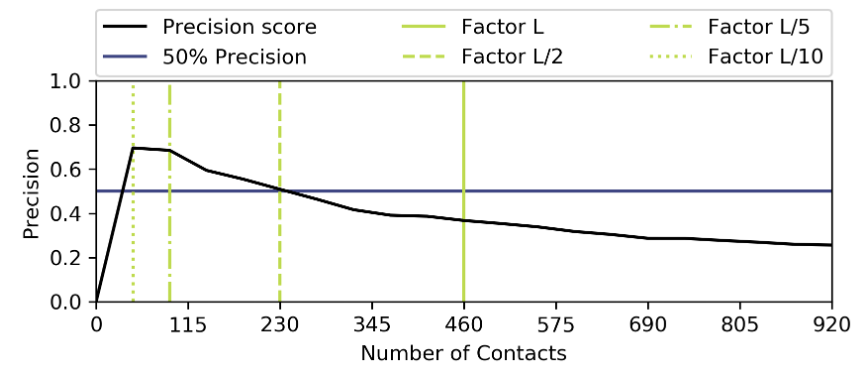
\includegraphics[width=\linewidth]{Modelling of Atg9/dmp_m2_prec.png}
  \caption{Precision profile of the Atg9 DMPFold model 2 against High Resolution Atg9 CryoEM Contacts}
  \label{fig:1}
\end{subfigure}\hfil % <-- added
\caption{Atg9 DMPFold Model 1 Quality Determination}
\small
\label{fig:atg9_dmp_m2_quality}
\end{figure}

The recent release of AlphaFold2 (AF2) \cite{Jumper2021} provided another opportunity to model Atg9. AF2 was able to construct a highly accurate model (Figure \ref{fig:af_6wqz}); aligning the model with the high resolution CryoEM structure 6wqz yielded a Z-score
of 50. This is a remarkable feet given that Atg9 has a new fold and AF2 was trained on the PDB in April 2018 when Atg9 was not present. The ability to model proteins where the fold has not been seen before has also been reported previously \cite{hegedHus2021alphafold2}.

\begin{figure}[th!]
    \centering
    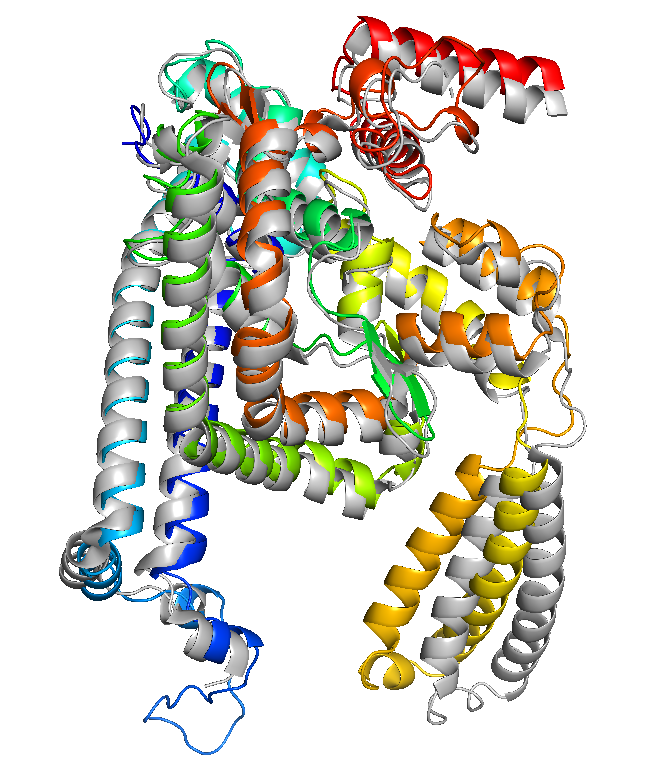
\includegraphics[width=50mm, scale=0.5]{Modelling of Atg9/af_6wqz.png}
    \caption{Superposition of AF2 model with CryoEM Atg9 (6wqz)}
    \label{fig:af_6wqz}
    \small
    AF2 model shown as rainbow (Blue: N-terminal to Red: C-terminal). CryoEM structure shown as grey.
\end{figure}

\newpage
\section{Conclusions}
The aim of the investigation into Atg9 was to build on the success of the Tmem41b study (Chapter 3) of using contact information to build plausible models and relate features of the models to function.  The attempt to structurally characterise Atg9 utilised contact information in three ways; comparing the crude homology models obtained by assuming an ABC-like fold with the predicted contact map directly, comparing the predicted contact map of Atg9 with actual contact maps of folds in the PDB (in addition to recently released CryEM models) and in making models.  Unlike Tmem41b, Atg9 is a large complex protein and successfully exploiting the methods utilised for Tmem41b proved difficult.  The eventual release of a high resolution model for Atg9 showed structural parallels with Tmem41b; the presence of re-entrant loops and a pseudo repeat.  However, unlike Tmem41b these features could not be deciphered through contact map analysis as Atg9 is much larger and complex in comparison to the DedA domain of Tmem41b.  A repeating set of contact map features could not be identified in the contact map of Atg9 as opposed to Tmem41b where a repeat in the form of contact map features is clearly visible. The re-entrant loops present in Atg9 are very unusual and have not been reported in any other solved structure.  Like Tmem41b these re-entrant loops have a conserved proline at their turning point and the residues on either side of this proline are highly conserved. However, in contrast to Tmem41b where the angle between the N-terminal and C-terminal halves of the re-entrant loops are around 20°, the N-terminal and C-terminal helices of the re-entrant loops in Atg9 are much wider apart and are not in contact therefore would not produce any contact map features.

An evolutionary relationship between the transmembrane region of Atg9 and the transmembrane region of Type I ABC transporters is a possibility given the sequence and structural similarities. Failure of the homology modelling is explainable knowing that two of the six ABC homologous transmembrane helices possess a large kink resulting in the formation of re-entrant loops in place of the equivalent transmembrane helices in Type I ABC transporters.  It would be plausible to hypothesise that Atg9 eveloved from Type 1 ABC transporters given the much broader species distribution of ABCs with Atg9 evolving much later. 


Currently most phylogenies of ABC transporters rely on the most conserved part of the protein which is the nucleotide binding domain and further investigation into the similarity between Type I ABC transporters and Atg9 is required to fully understand the evolutionary relationship between them. 

Although a high resolution model now exists for Atg9, the availability of new highly accurate protein structure prediction methods such as AlphaFold will allow the opportunity to model Atg9 protein-protein complexes to aid the understanding of Atg9 behaviour.  Atg9 is known to interact with a variety of proteins in the process of autophagasome construction such as ULK1, Atg2 as well modulating elements of the primary immune response through its interaction with STING \cite{li2019tmem203}.  Attempted Alphafold modelling of these complexes may help to provide evidence of whether these interactions are indeed direct or whether other proteins mediate the interaction.
%use AF to model complex with STING ...don't use template in case it forces into 1 conformation




